\documentclass[12pt,a4paper]{report}
\usepackage{lipsum}% http://ctan.org/pkg/lipsum
\usepackage{titletoc}% http://ctan.org/pkg/titletoc
\usepackage[T1]{fontenc}
\usepackage{natbib}
\usepackage{url}
\usepackage{titlesec}
\usepackage{graphicx}
\usepackage{subfig}
\usepackage{array}% http://ctan.org/pkg/array
\usepackage{placeins}
\usepackage{amsmath,amssymb}
\usepackage{booktabs, makecell}
\usepackage{siunitx, mhchem}
\usepackage{enumitem}

\usepackage{layout}
\setlength{\voffset}{-0.5in}
\setlength{\headsep}{5pt}
\def\x#1{\texttt{\expandafter\string\csname#1\endcsname}&\expandafter$\csname#1\endcsname$}

\newenvironment{tightcenter}{%
  \setlength\topsep{0pt}
  \setlength\parskip{0pt}
  \begin{center}
}{%
  \end{center}
}

\usepackage{float}
\graphicspath{ {images/} }
\tolerance=1
\emergencystretch=\maxdimen
\hyphenpenalty=10000
\hbadness=10000  
\titleformat{\chapter}{\normalfont\huge}{\thechapter.}{20pt}{\huge}
\titlespacing*{\chapter}{0pt}{0pt}{20pt}


\begin{document}
\begin{titlepage}
	\centering
	{\scshape\LARGE University of Bath \par}
	\vspace{1cm}
	{\scshape\Large Literature Review\par}
	\vspace{1.5cm}
	{\huge\bfseries The Development of a Serious Game to Teach Aristotle's Syllogisms\par}
	\vspace{2cm}
	{\Large\itshape James Treasure\par}
	\vfill
	supervised by\par
	Dr.~Willem \textsc{Heijltjes}
	\vfill
	{\large \today\par}
\end{titlepage}

\tableofcontents
\chapter{Syllogisms}
\section{History}

Aristotle's work on formal logic was the earliest known study of the topic, which remained at the forefront of academia until the 19th century following Gotlobb Frege's work on first order logic. As syllogisms were so prominent for such a long period of time they have had huge cultural significance on logic in the Western world \citep{sep-aristotle-logic}. Up until the 12th century medieval logicians only had access to a small portion of Aristotle's work with the notable exclusion being Prior Analytics, which contained his work on syllogisms. This period of time is known as logica vetus, or old logic, and it wasn't until the 12th century when Prior Analytics resurfaced in the west that the logica nova, or new logic, began. Immanuel Kant, a prominent 18th century philosopher, went as far as to describe Prior Analytics as "a closed and completed body of doctrine" demonstrating just how highly Aristotle's work on syllogisms was thought of.

\section{What are syllogisms}
Aristotle defined his syllogisms as \textit{a discourse in which, certain things having been supposed, something different from the things supposed results of necessity because these things are so}. Put more simply syllogisms are a type of deductive reasoning that, when used on a logical argument, allows a conclusion to be drawn. Aristotle's focus was on categorical syllogisms, essentially a  logical argument that contains three categorical propositions. These three categorical propositions in turn are made up of two premises and a conclusion. Each categorical premise is made up of categorical terms, of which each is used twice in the syllogism as a whole. Each categorical premise can be described as a sentence that connects a predicate and a subject by a verb. 
\bigbreak
\begin{tightcenter}
\textit{All M are P} $\rightarrow$ major premise\\
\textit{All S are M} $\rightarrow$ minor premise\\
\textit{All S are P} $\rightarrow$ conclusion \\
\end{tightcenter}
\bigbreak
Syllogisms are capable of being applied to any logical argument but to allow them to be compared to each other, they must be represented in a standard form. A categorical syllogism that follows standard form is always structured in the same way, first the major premise, then the minor premise followed by the conclusion. 

As created by medieval logicians studying Aristotle's work, the mood and figure of a syllogism provides a notation to represent all the logically unique variations that can occur. The mood refers to the order in which the categorical propositions appear in the syllogism and is represented by four different classes.%
\begin{itemize}
\item \textbf{A} - All A is B $\rightarrow$ universal affirmative proposition
\item \textbf{I} - Some A is B $\rightarrow$ particular affirmative proposition
\item \textbf{E} - No A is B $\rightarrow$ universal negative  proposition
\item \textbf{O} - Some A is not B  $\rightarrow$  particular negative proposition
\end{itemize}
Syllogisms also have a figure that describes the placement of the two middle terms.

\begin{center}
  \begin{tabular}{ l | c | c | c | r }
     & Figure 1 & Figure 2 & Figure 3 & Figure 4 \\ \hline
    Major & M-P & P-M & M-P & P-M \\ \hline
    Minor & S-M & S-M & M-S & M-S \\
  \end{tabular}
\end{center}

By combining all the different possibilities of mood and figure there are 256 logically unique syllogisms, eg., AOO-2. 
\bigbreak
\begin{tightcenter}
\textit{All P is M}\\ 
\textit{Some S is not M}\\
\textit{Some S is not P}\\
\end{tightcenter}
\bigbreak

Only 24 syllogisms out of the possible 256 are logically valid, and of these the existential fallacy is broken by 15 of them.

\subsection{Existential Fallacy}

The existential fallacy occurs whenever an argument is invalid because the premises lack existential import. Existential import is an attribute of a categorical proposition that implies the existence of the subject \citep{hurley2005concise}. There are two schools of thought on the existential fallacy with regards to syllogism, Aristotelian and Boolean.

Traditionally, as laid out by Aristotle, the existence of a subject is assumed when making universal statements. I and O propositions are said to have existential import and in Aristotelian logic I and O propositions must follow from A and E propositions due to subalternation. Subalternation is an inference made between A and I or E and O propositions. It says that if A is true it can be inferred I is true, similarly with E and O. This leads to A and E propositions also having existential import as a proposition with existential import cannot be derived from a proposition without existential import.
By considering the syllogism in figure 1.1 we can say that it does not commit the existential fallacy as dogs do exist whereas in figure 1.2 the existential fallacy is committed as dragons do not exist. 

However, as modern day logicians and mathematicians often reason about empty sets or imaginary objects the Aristotelian approach to the existential fallacy was problematic. George Boole, a 19th century philosopher, built upon Aristotle's work to create his own Boolean syllogisms to address this issue by stating that universal propositions do not have existential import, thus allowing empty sets \citep{hammerhill}. In Boolean syllogisms both figure \ref{fig:existenetialFallacy1} and \ref{fig:existenetialFallacy2} commit the existential fallacy.


\begin{figure}[!h]
  \centering
  \begin{minipage}[b]{0.4\textwidth}
    \begin{tightcenter}
		\textit{All dogs are mammals }\\ 
		\textit{All mammals are animals}\\
		\textit{Some dogs are animals}\\
		\end{tightcenter}
		    \caption{}
		    \label{fig:existenetialFallacy1}
  \end{minipage}
  \hfill
  \begin{minipage}[b]{0.4\textwidth}
    \begin{tightcenter}
		\textit{All gorillas are lizards }\\ 
		\textit{All dragons are lizards}\\
		\textit{Some dragons are not gorillas}\\
		\end{tightcenter}
				    \caption{}
		    \label{fig:existenetialFallacy2}
  \end{minipage}
\end{figure}
\FloatBarrier

The general rule to reason if a syllogism the commits existential fallacy is that if both premises are universal then the conclusion cannot be particular. In Boolean logic if this rule is broken, then it is a fallacy but in Aristotelian logic the rule must be broken and the critical term must also not exist.

\section{Current teaching}
Syllogisms currently feature almost exclusively on philosophy courses around the world, typically as part of units on formal logic. However, Venn Diagrams are taught to children in primary school and set theory features on most maths and computer science degrees. So whilst they are not directly taught about syllogisms, they are already familiar with some of the most common ways to represent them.
There are a few different ways that are currently used to represent syllogisms when teaching, with most courses using a mixture of sentential, set theory notation and diagrams. 
It is common to initially introduce syllogisms in sentential form, using real world examples as opposed to letters. The advantage of this is it becomes far easier for the learner to visualise the propositions. For example, visualising the statement "all dogs are animals" is simpler than "all A are B" despite being representing the same idea. 

However representing syllogisms this way is not the most effective as they can be logically quite complex. As \citep{larkin1987diagram} explains, sentential form requires inferences to be made, and then those inferences to be held in memory. Working through the syllogism, for example to decide if it is valid, means that these inferences must be continually remembered. As shown by \cite{johnson1980mental}, sentential forms of syllogism are more difficult to understand and may be mentally translated into diagrammatic representations internally anyway. 

\subsection{Venn Diagrams}
Venn diagrams are the most commonly used diagrammatic representation of syllogisms. The advantage over other diagrammatic forms is that most people have been taught them at a young age and are therefore very familiar with them. 

In this representation each circle is a term, which is then filled in to represent the empty set or marked with a X to show at least one member. To achieve the final diagram the two previous diagrams are combined which can then  be used to check the validity of the syllogism. It can be seen from table \ref{tbl:vennEAO-3} that even complex syllogisms are able to be represented with relatively little complexity using Venn diagrams which contributes to their popularity. 

\begin{table}[h!]
  \centering
  \begin{tabular}{  c  c  c  c }
    A & I & E & O\\
    \begin{minipage}{.22\textwidth}
      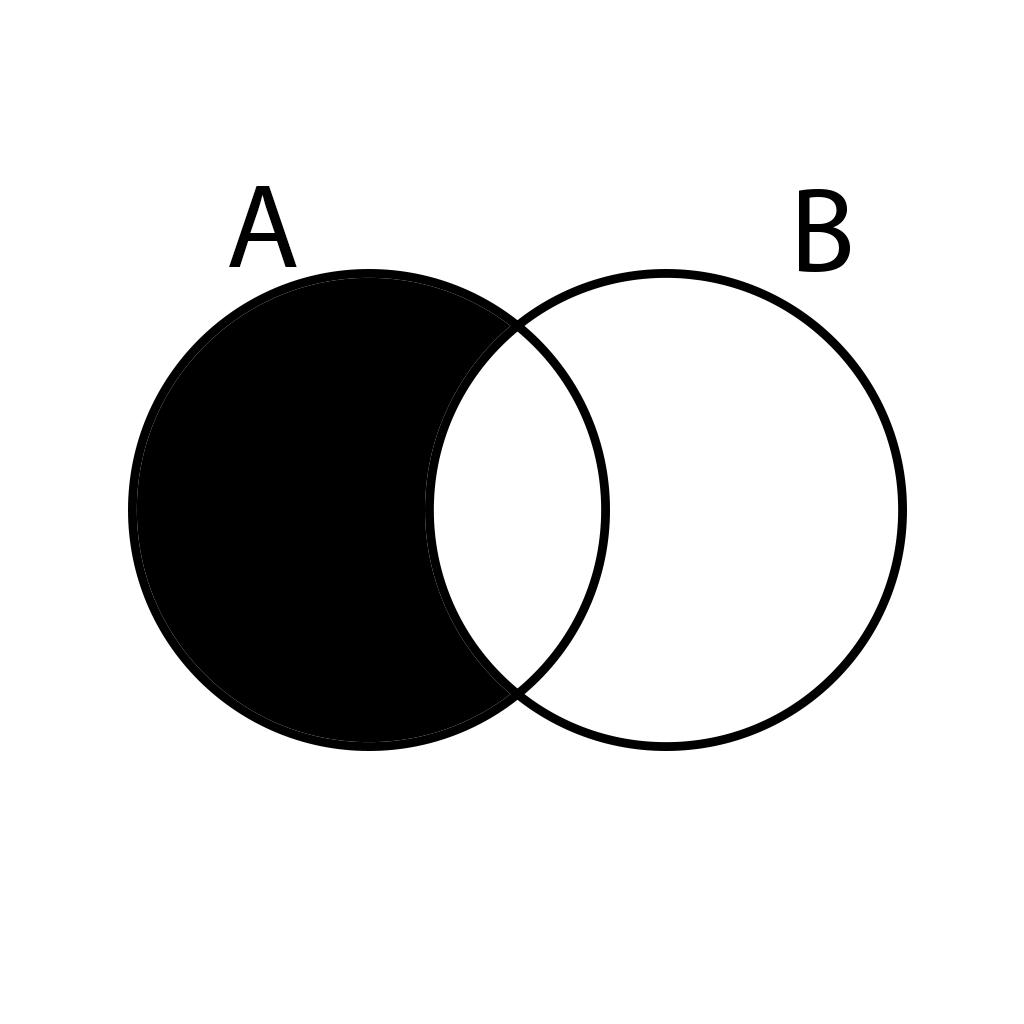
\includegraphics[width=\linewidth]{AVenn}
    \end{minipage}
    &
    \begin{minipage}{.22\textwidth}
      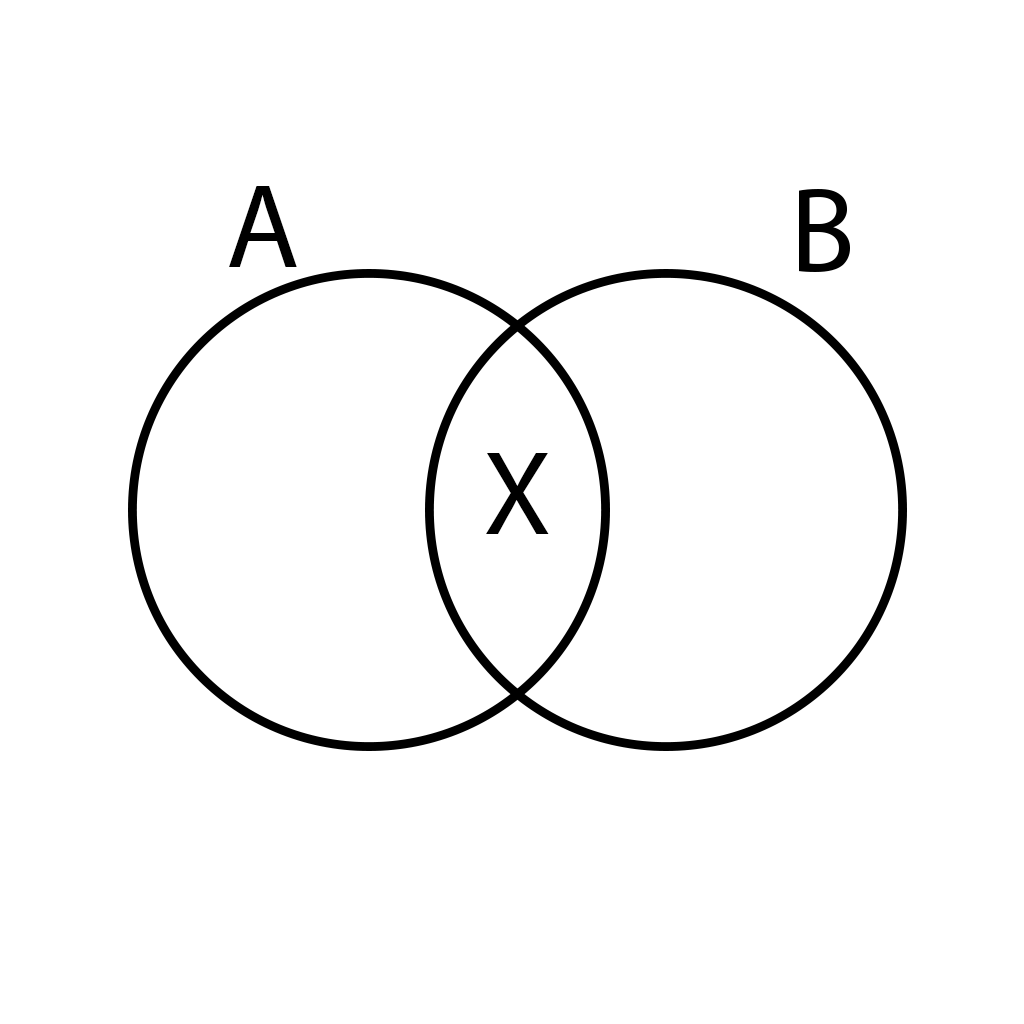
\includegraphics[width=\linewidth]{IVenn}
    \end{minipage}
    & 
    \begin{minipage}{.22\textwidth}
      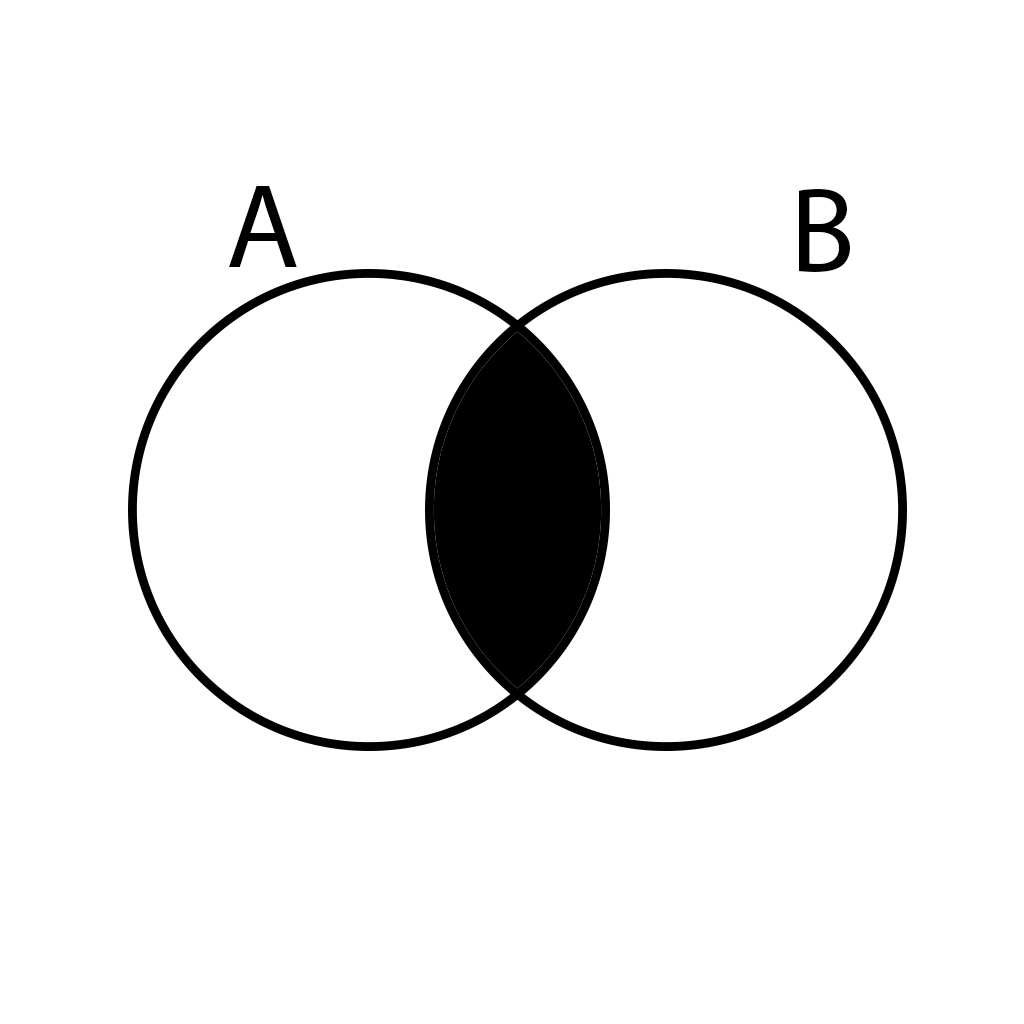
\includegraphics[width=\linewidth]{EVenn}
    \end{minipage}
    &
    \begin{minipage}{.22\textwidth}
      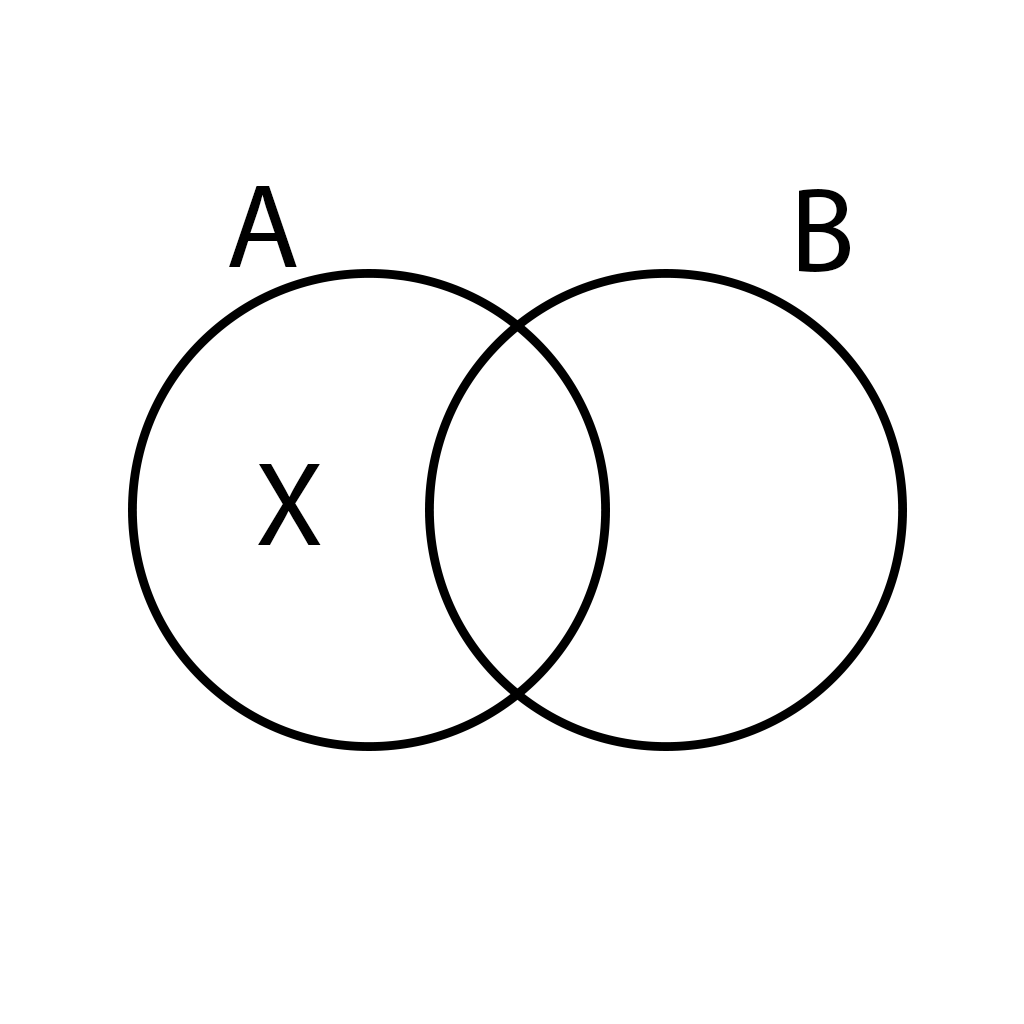
\includegraphics[width=\textwidth]{OVenn}
    \end{minipage}
    \\
  \end{tabular}
  \caption{Premises represented by Venn Diagrams}\label{tbl:vennPremises}
\end{table}

\begin{table}[htb]
  \centering
\begin{tabular}{>{\raggedright\arraybackslash}m{40mm} m{40mm} m{40mm}}
    \multicolumn{1}{>{\centering\arraybackslash}m{40mm}}{\textbf{All Men Are Mortal}} 
    & \multicolumn{1}{>{\centering\arraybackslash}m{40mm}}{\textbf{All Greeks Are Men}} 
    & \multicolumn{1}{>{\centering\arraybackslash}m{40mm}}{\textbf{All Greeks Are Mortal}}\\

    \begin{minipage}{.29\textwidth}
    \begin{center}
      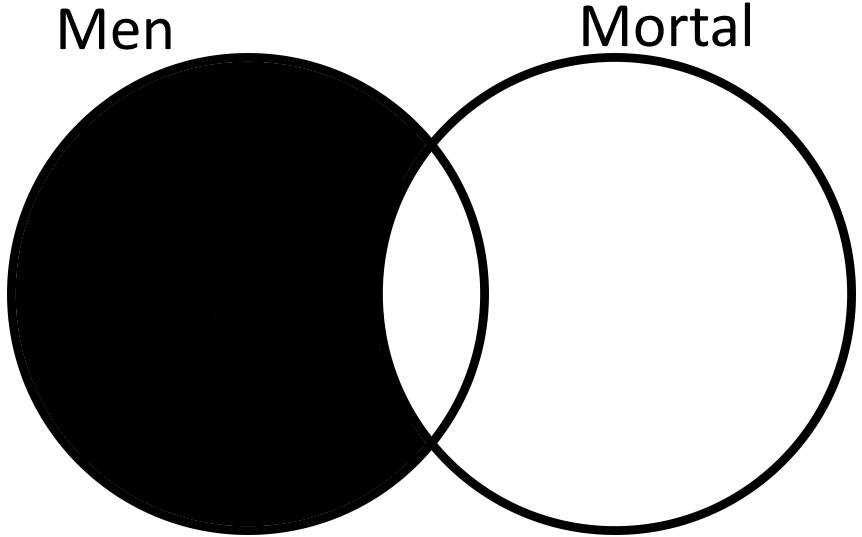
\includegraphics[scale=0.25]{VennAllMenAreMortal}
    \end{center}
      
    \end{minipage}
    &
    \begin{minipage}{.29\textwidth}
    \begin{center}
      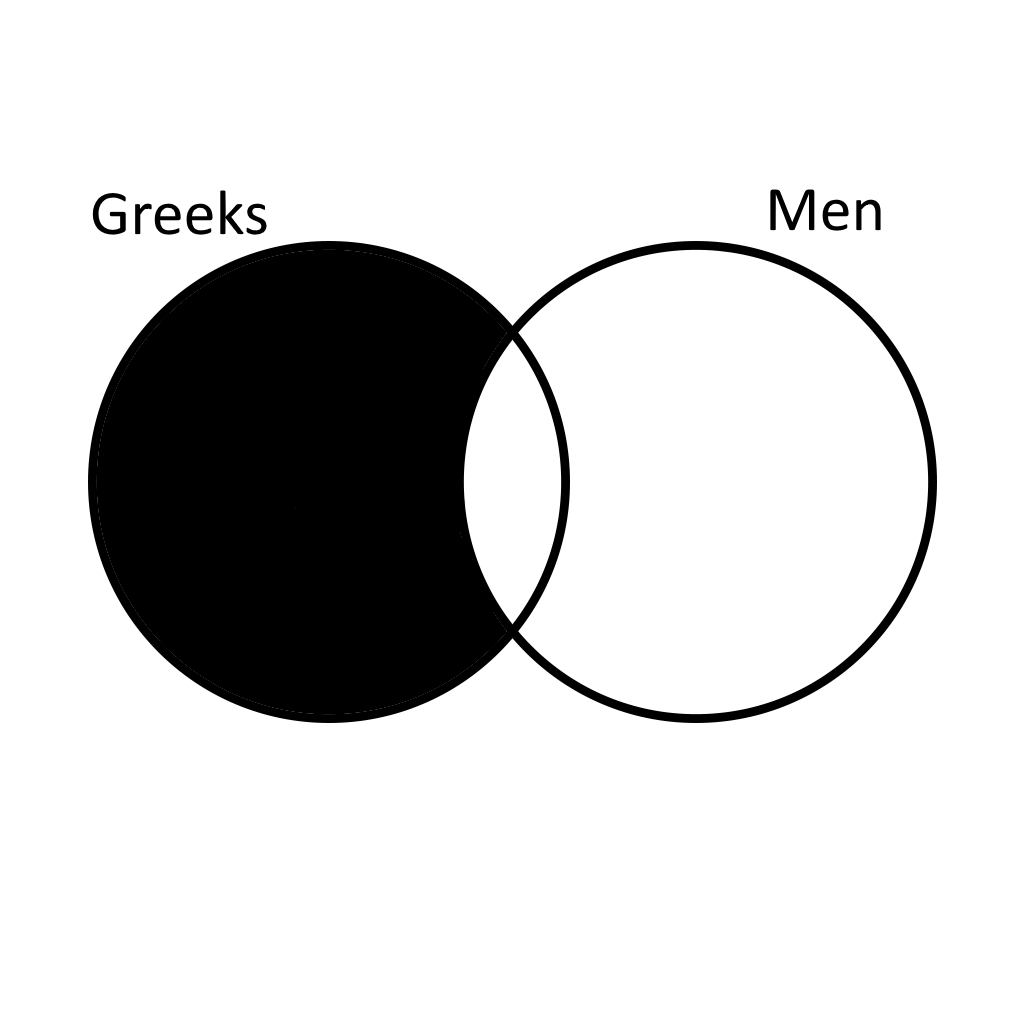
\includegraphics[scale=0.25]{VennAllGreeksAreMen}
    \end{center}
      
    \end{minipage}
    & 
    \begin{minipage}{.29\textwidth}
    \begin{center}
      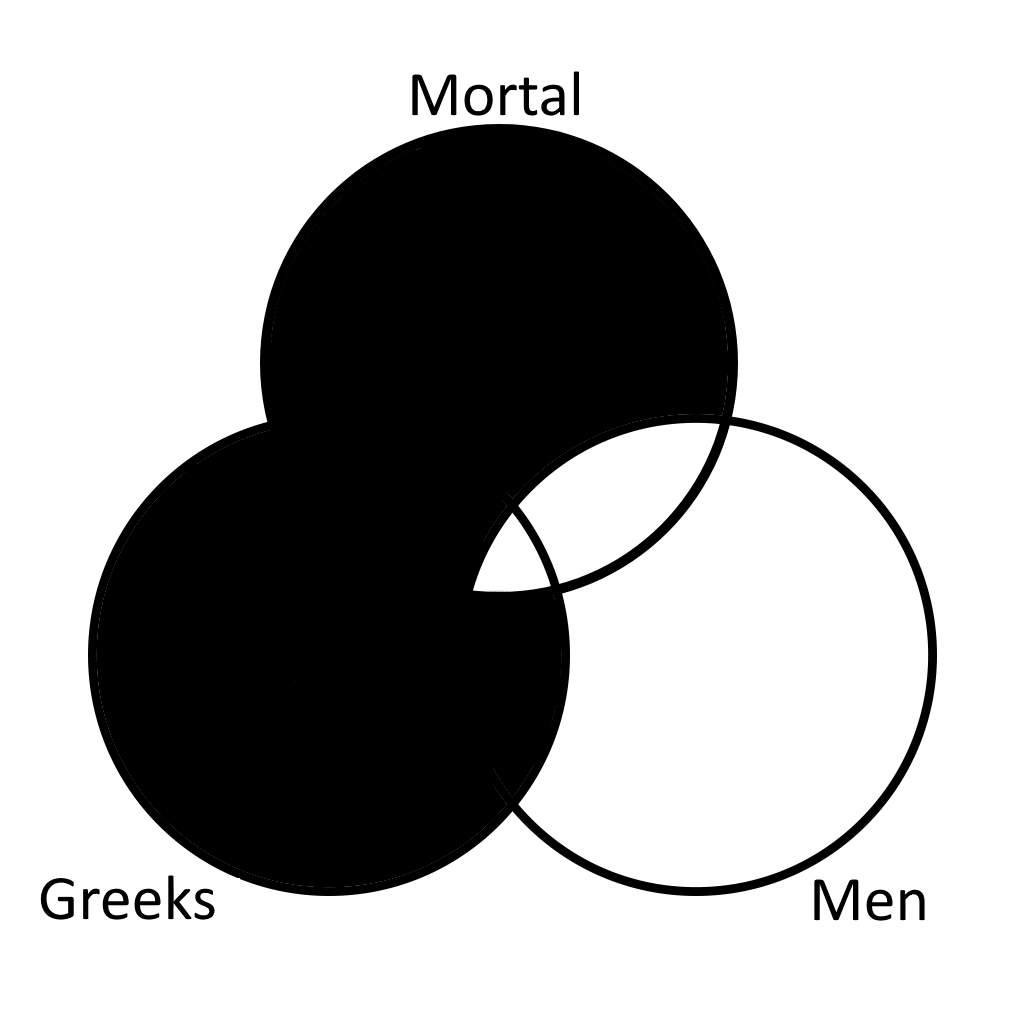
\includegraphics[scale=0.16]{VennAllGreeksAreMortal}
    \end{center}
  
    \end{minipage}
    \\
  \end{tabular}
  \caption{AAA-1 Syllogism}\label{tbl:vennAAA-1}
\end{table}
\FloatBarrier

\begin{table}[htb]
  \centering
\begin{tabular}{>{\raggedright\arraybackslash}m{40mm} m{40mm} m{40mm}}
    \multicolumn{1}{>{\centering\arraybackslash}m{40mm}}{\textbf{No lizards are mammals}} 
    & \multicolumn{1}{>{\centering\arraybackslash}m{40mm}}{\textbf{All lizards are reptiles}} 
    & \multicolumn{1}{>{\centering\arraybackslash}m{40mm}}{\textbf{Some reptiles are not mammals}}\\
    \begin{minipage}{.29\textwidth}
    \begin{center}
    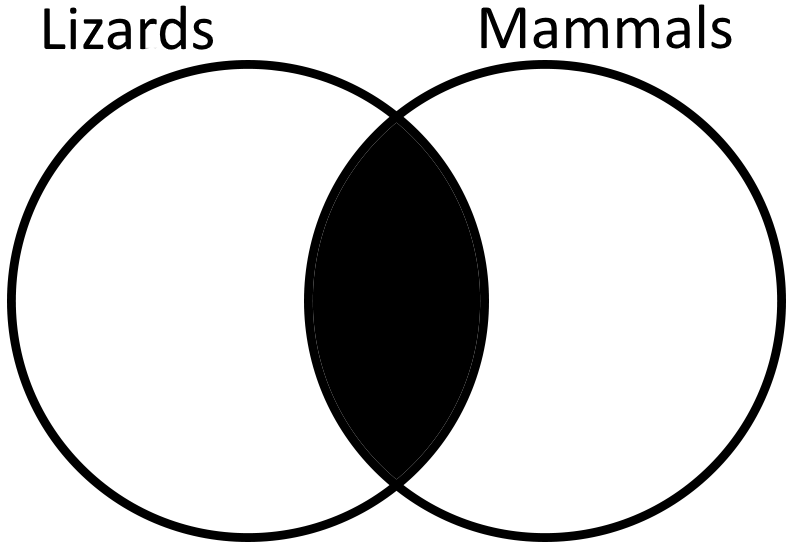
\includegraphics[scale=0.25]{VennNoLizardsAreMammals}
    \end{center}
      
    \end{minipage}
    &
    \begin{minipage}{.29\textwidth}
    \begin{center}
    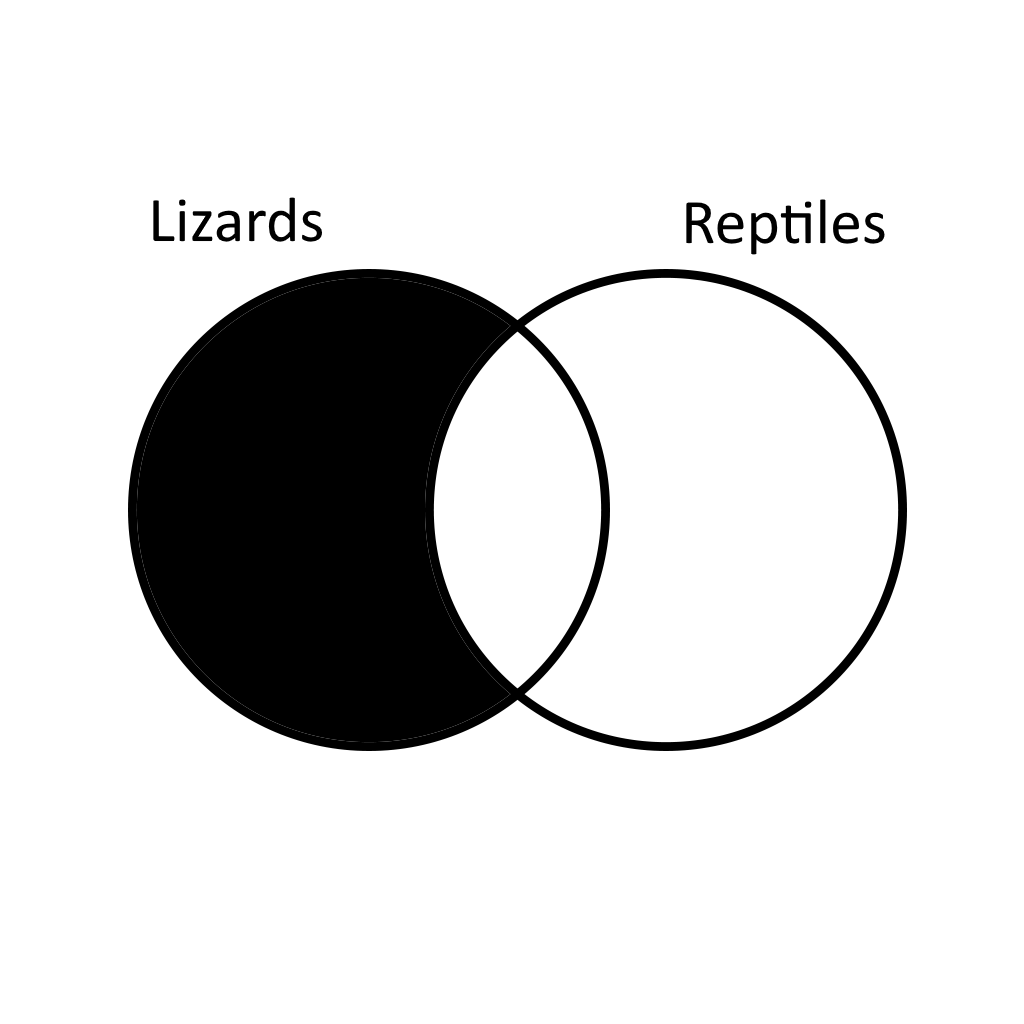
\includegraphics[scale=0.25]{VennAllLizardsAreReptiles}
    \end{center}
      
    \end{minipage}
    & 
    \begin{minipage}{.29\textwidth}
    \begin{center}
     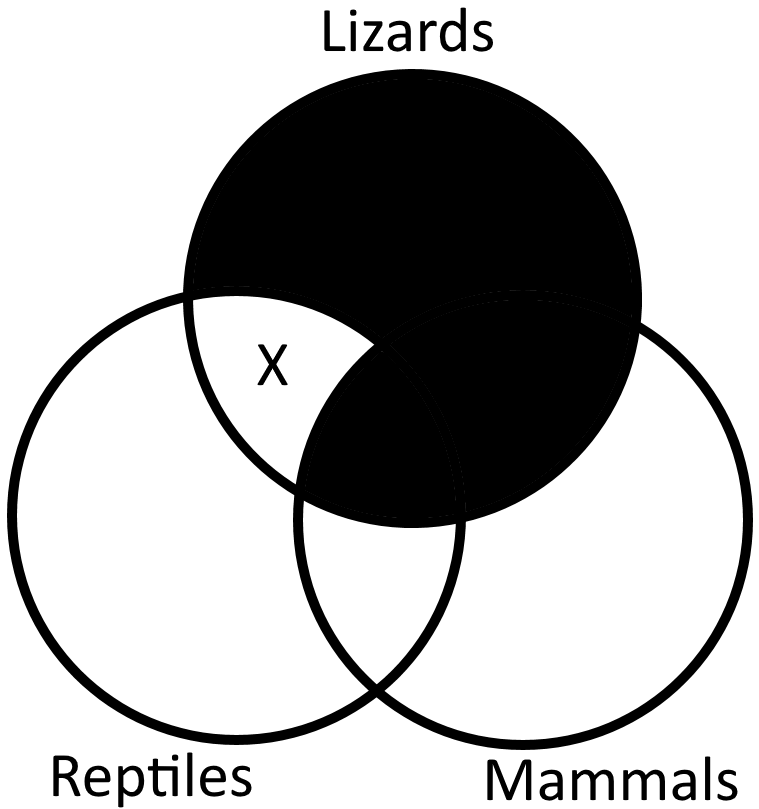
\includegraphics[scale=0.25]{VennSomeReptilesAreNotMammals}
    \end{center}
  
    \end{minipage}
    \\
  \end{tabular}
  \caption{EAO-3 Syllogism}\label{tbl:vennEAO-3}
\end{table}
\FloatBarrier



\subsection{Euler Circles}
Euler circles are another popular way in which syllogisms can be represented. 
These are a very natural way of representing sets, with \cite{Erickson1978-ERIROS} putting forward the theory that when people are thinking about syllogisms that they are in fact being mentally thought of as Euler circles. As table \ref{tbl:eulerPremises} shows, when used to represent the individual premises Euler circles can be very intuitive.

%Cirles are 8.5cm I think
\begin{table}[h!]
  \centering
  \begin{tabular}{  c  c  c  c }
    A & I & E & O\\
    \begin{minipage}{.22\textwidth}
      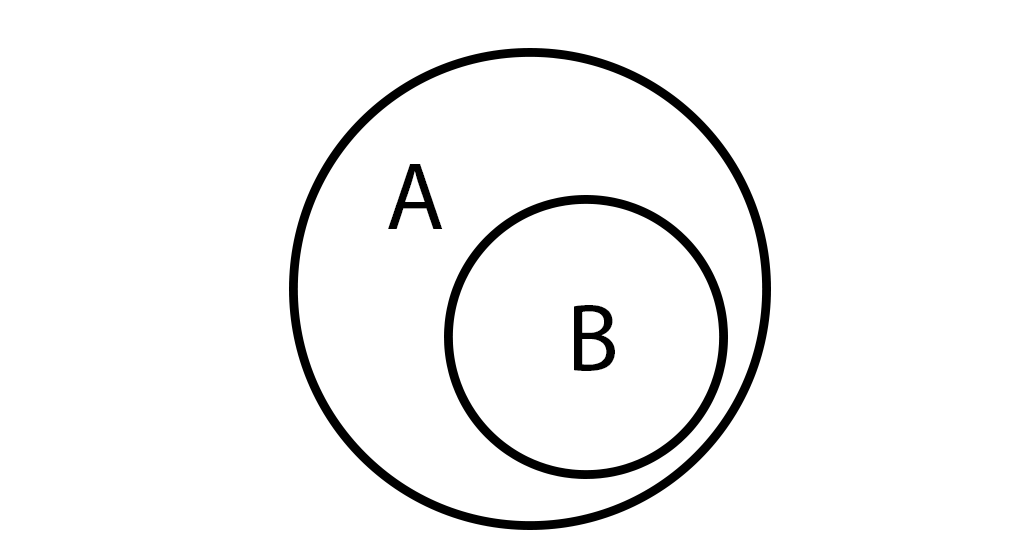
\includegraphics[width=\linewidth]{AEuler}
    \end{minipage}
    &
    \begin{minipage}{.22\textwidth}
      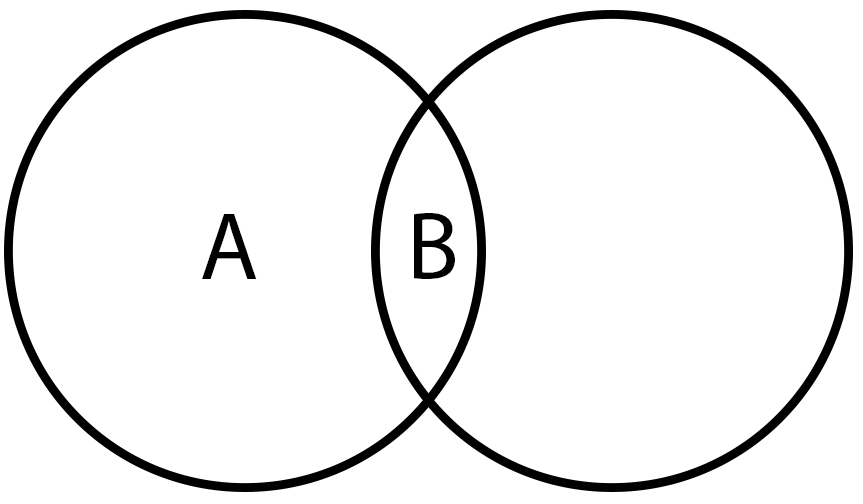
\includegraphics[width=\linewidth]{IEuler}
    \end{minipage}
    & 
    \begin{minipage}{.22\textwidth}
      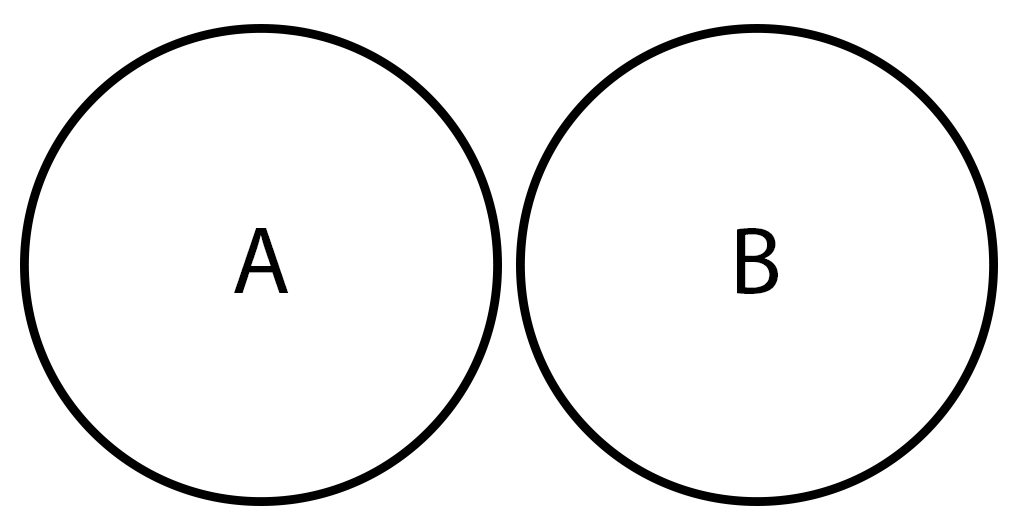
\includegraphics[width=\linewidth]{EEuler}
    \end{minipage}
    &
    \begin{minipage}{.22\textwidth}
      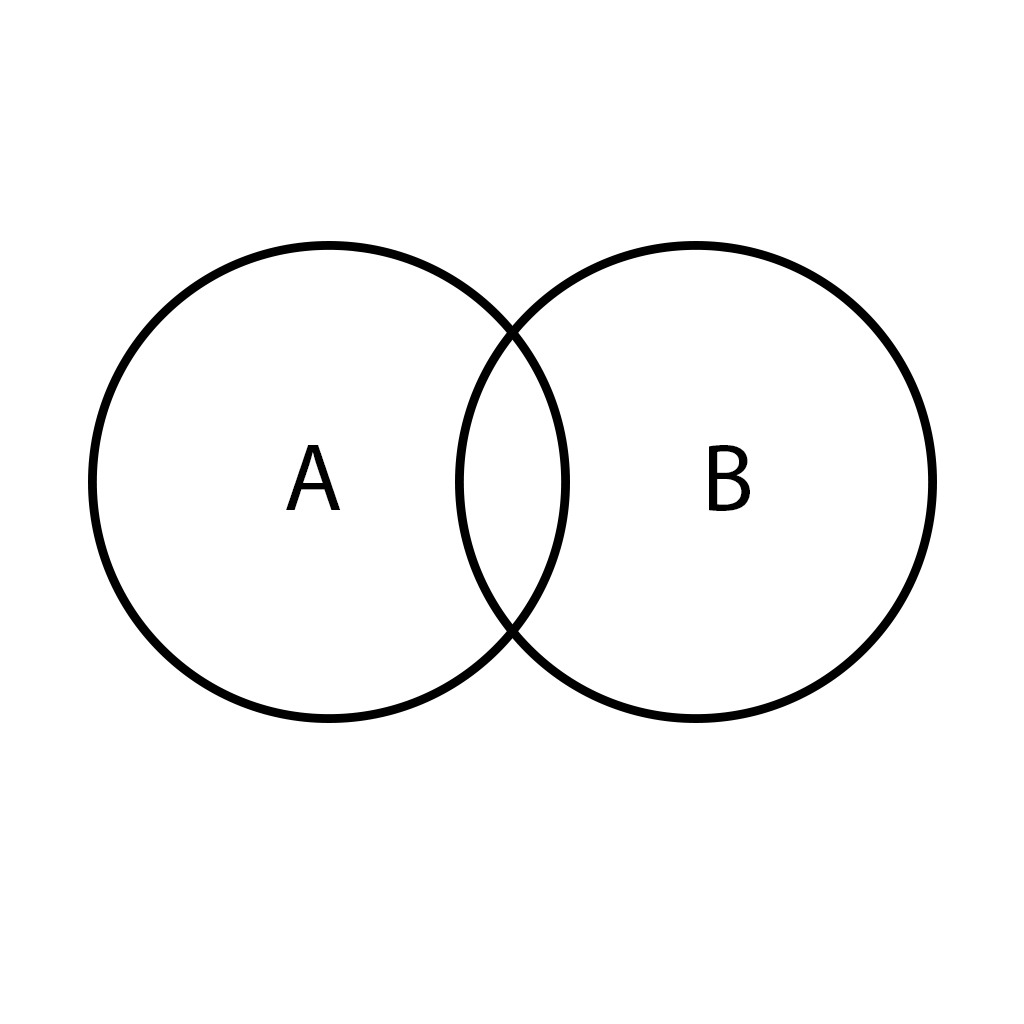
\includegraphics[width=\textwidth]{OEuler}
    \end{minipage}
    \\
  \end{tabular}
  \caption{Premises represented by Euler Circles}\label{tbl:eulerPremises}
\end{table}



\begin{table}[htb]
  \centering
  \begin{tabular}{ c  c  c }
    All Men Are Mortal & All Greeks Are Men & All Greeks Are Mortal\\
    \begin{minipage}{.29\textwidth}
        \begin{center}
             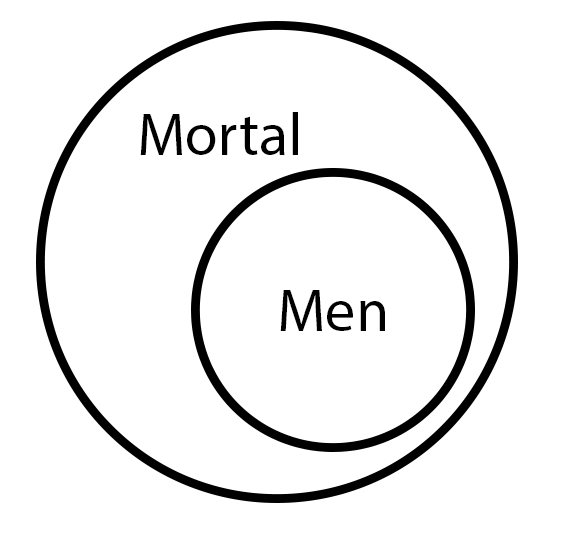
\includegraphics[scale=0.25]{EulerAllMenAreMortal}
         \end{center}
    \end{minipage}
    &
    \begin{minipage}{.29\textwidth}
         \begin{center}
              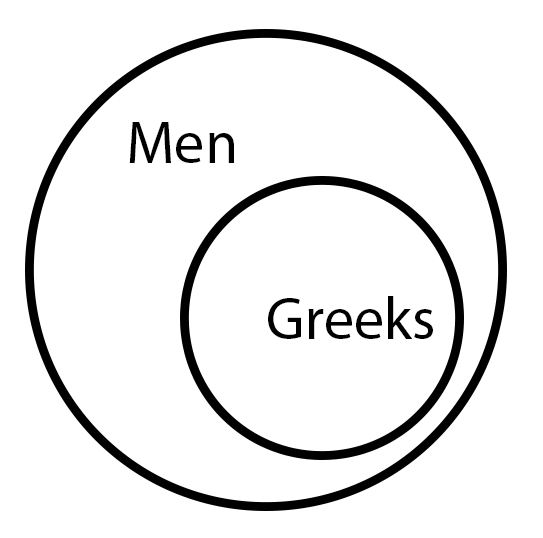
\includegraphics[scale=0.25]{EulerAllGreeksAreMen}
         \end{center}
    \end{minipage}
    & 
    \begin{minipage}{.29\textwidth}
         \begin{center}
         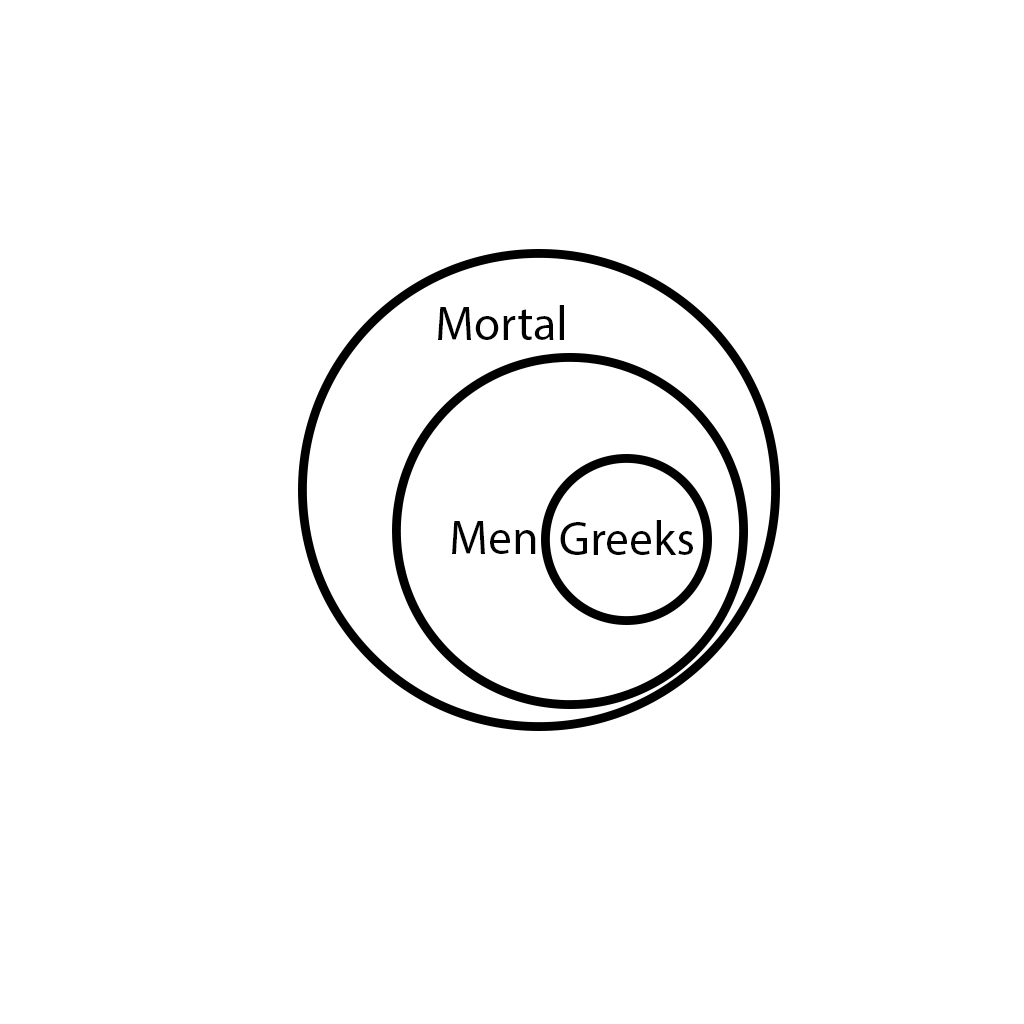
\includegraphics[scale=0.25]{EulerAllGreeksAreMortal}
    \end{center}
    \end{minipage}
    \\
  \end{tabular}
  \caption{Premises represented by Euler Circles}\label{tbl:eulerAllMenMortal}
\end{table}
\FloatBarrier
Euler circles also concisely represents simpler syllogisms as table \ref{tbl:eulerAllMenMortal} shows. However, the problem with this representation arises when more complex syllogisms are constructed. When there are multiple ways to represent the conclusion the result needs more than one diagram to depict all of the possibilities as seen in table \ref{tbl:eulerHomework} . It is at this point that the intuitive benefits are quickly outweighed by the added overhead of managing multiple conclusive diagrams.

\begin{table}[h!]
  \centering
  \begin{tabular}{  c  c  c }
    No homework is fun & Some reading is homework & Some reading is not fun\\
    \begin{minipage}{.22\textwidth}
      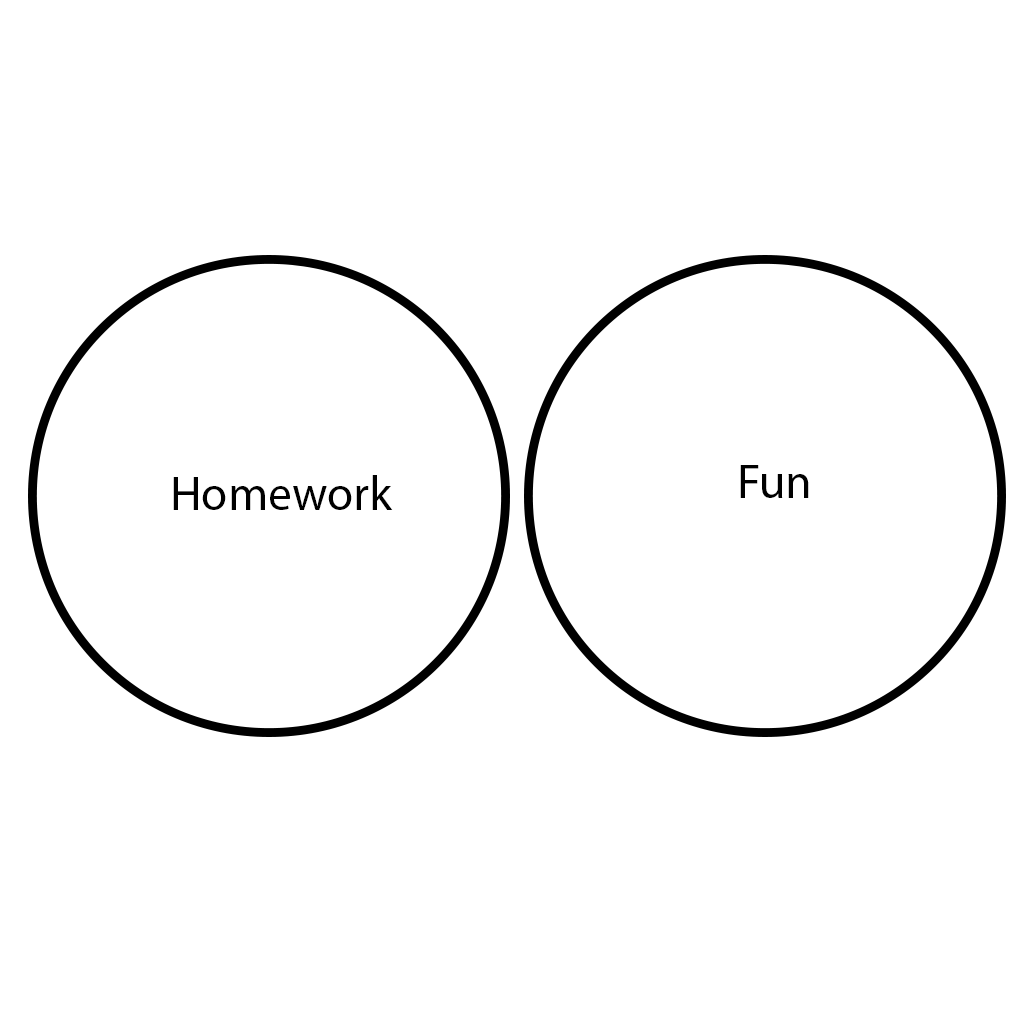
\includegraphics[width=\linewidth]{EulerNoHomeworkFun}
    \end{minipage}
    &
    \begin{minipage}{.22\textwidth}
      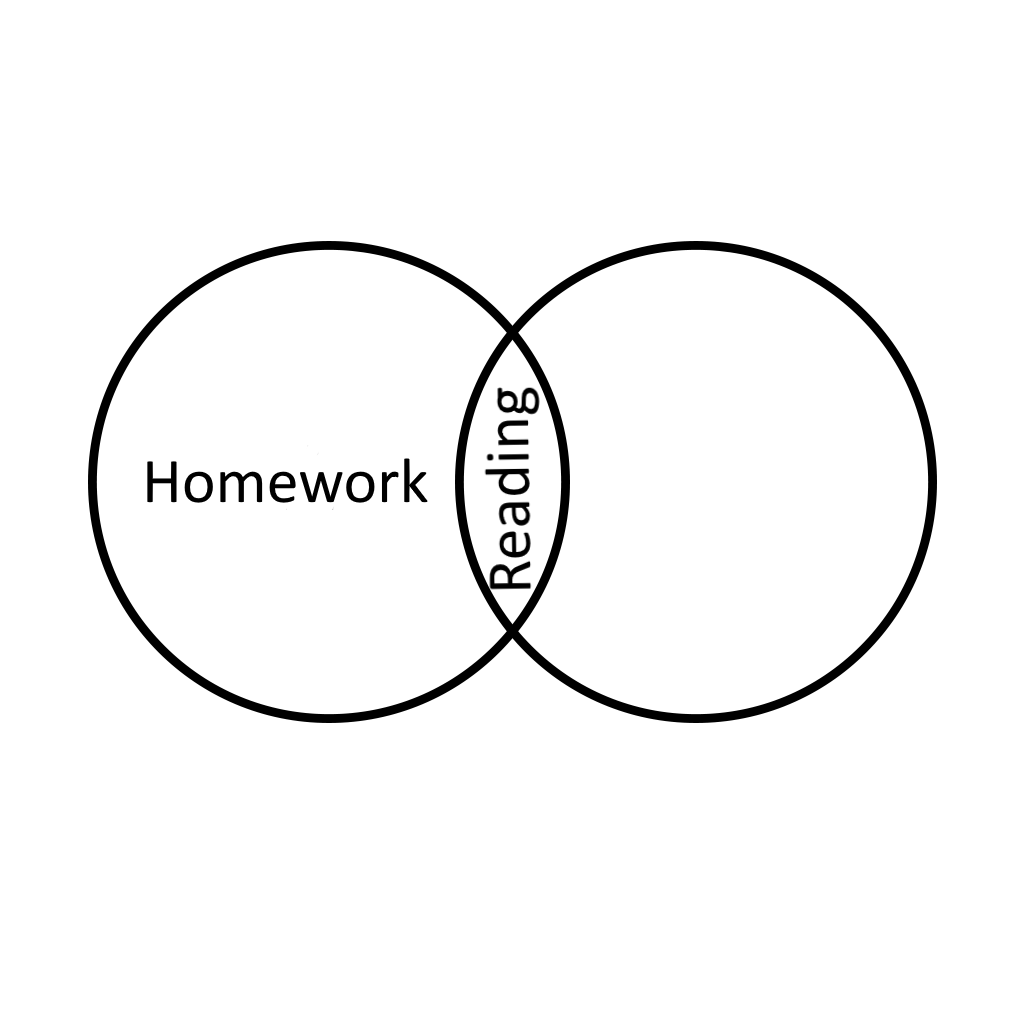
\includegraphics[width=\linewidth]{EulerSomeReadingIsHomework}
    \end{minipage}
    & 
    \begin{minipage}{.22\textwidth}
      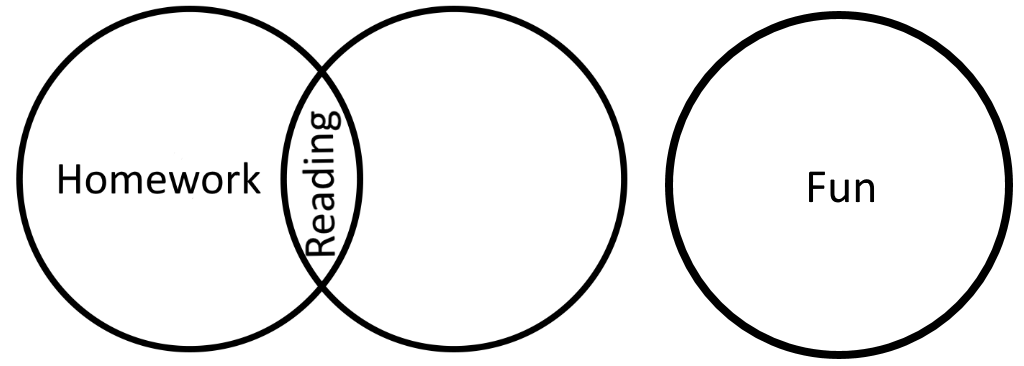
\includegraphics[width=\linewidth]{EulerSomeReadingIsNotFun1}
    \end{minipage}
    \\
    &
     &
    \begin{minipage}{.22\textwidth}
      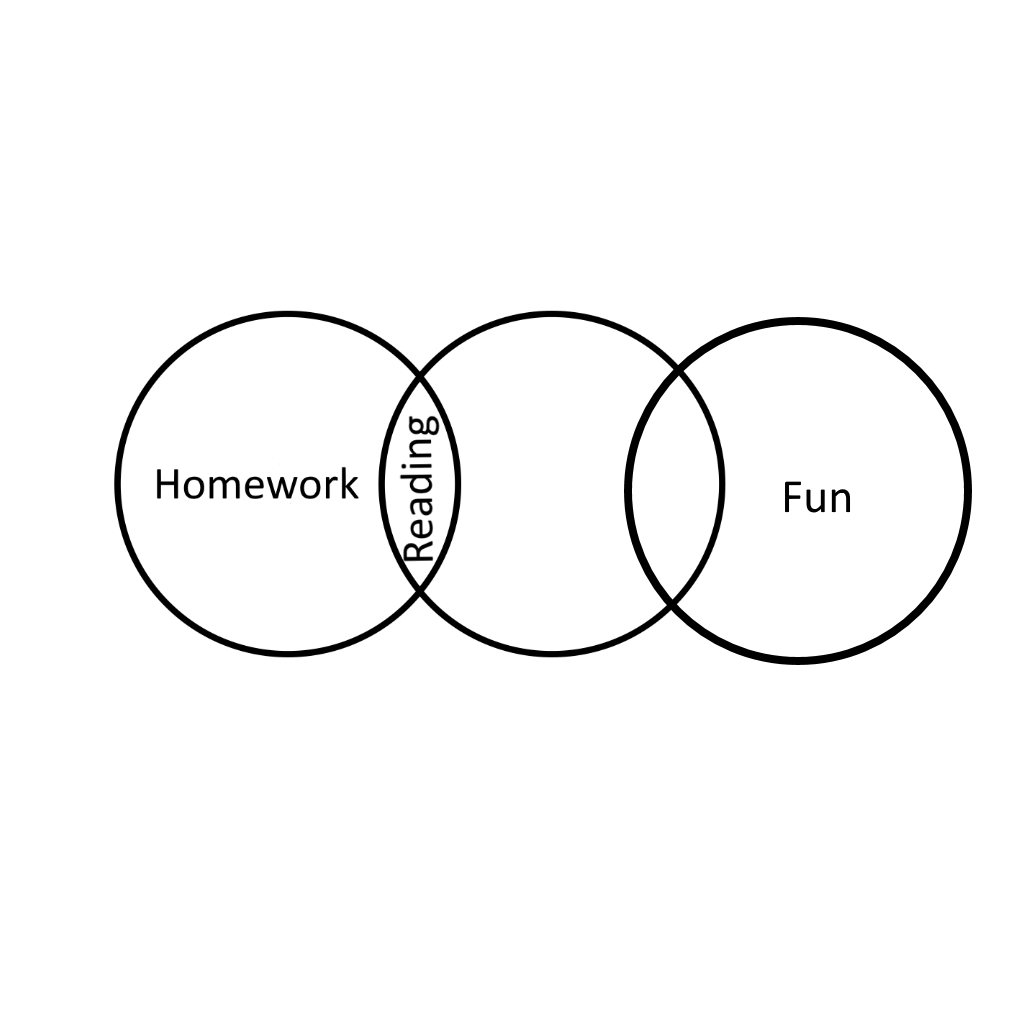
\includegraphics[width=\textwidth]{EulerSomeReadingIsNotFun2}
    \end{minipage}
    \\
    &
     &
    \begin{minipage}{.22\textwidth}
      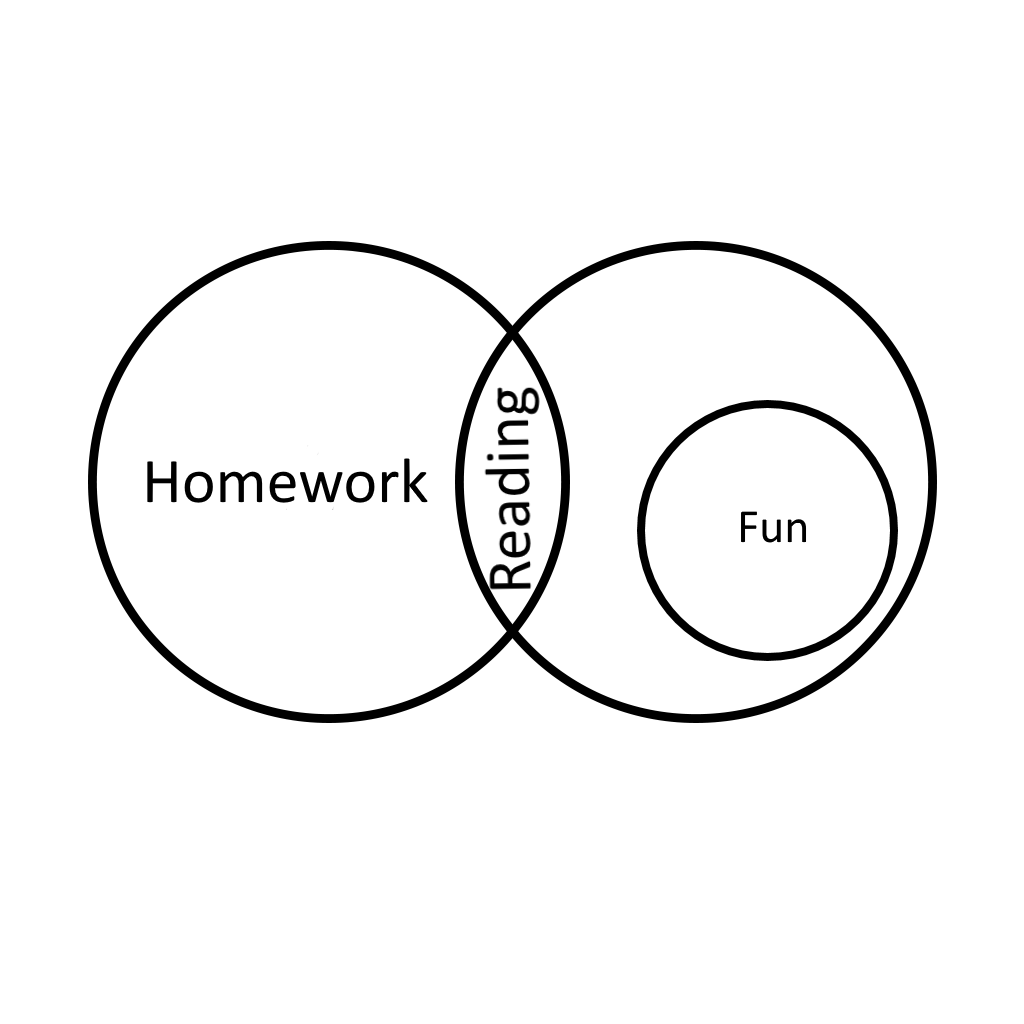
\includegraphics[width=\textwidth]{EulerSomeReadingIsNotFun3}
    \end{minipage}
    \\
  \end{tabular}
  \caption{EIO Syllogism}\label{tbl:eulerHomework}
\end{table}
\FloatBarrier


\subsection{Linear Diagrams}
Linear diagrams are an alternative system that was devised by \cite{englebretsen1991}. As the name suggests they are linear instead planar like Venn and Euler diagrams. The reasoning behind this was that Englebretsen said it allowed linear diagrams to represent 4 terms, unlike their planar counterparts. Elements are represented by points which are then connected by lines to show sets.

%Cirles are 8.5cm I think
\begin{table}[h!]
  \centering
  \begin{tabular}{  c  c  c  c }
    A & I & E & O\\
    \begin{minipage}{.22\textwidth}
      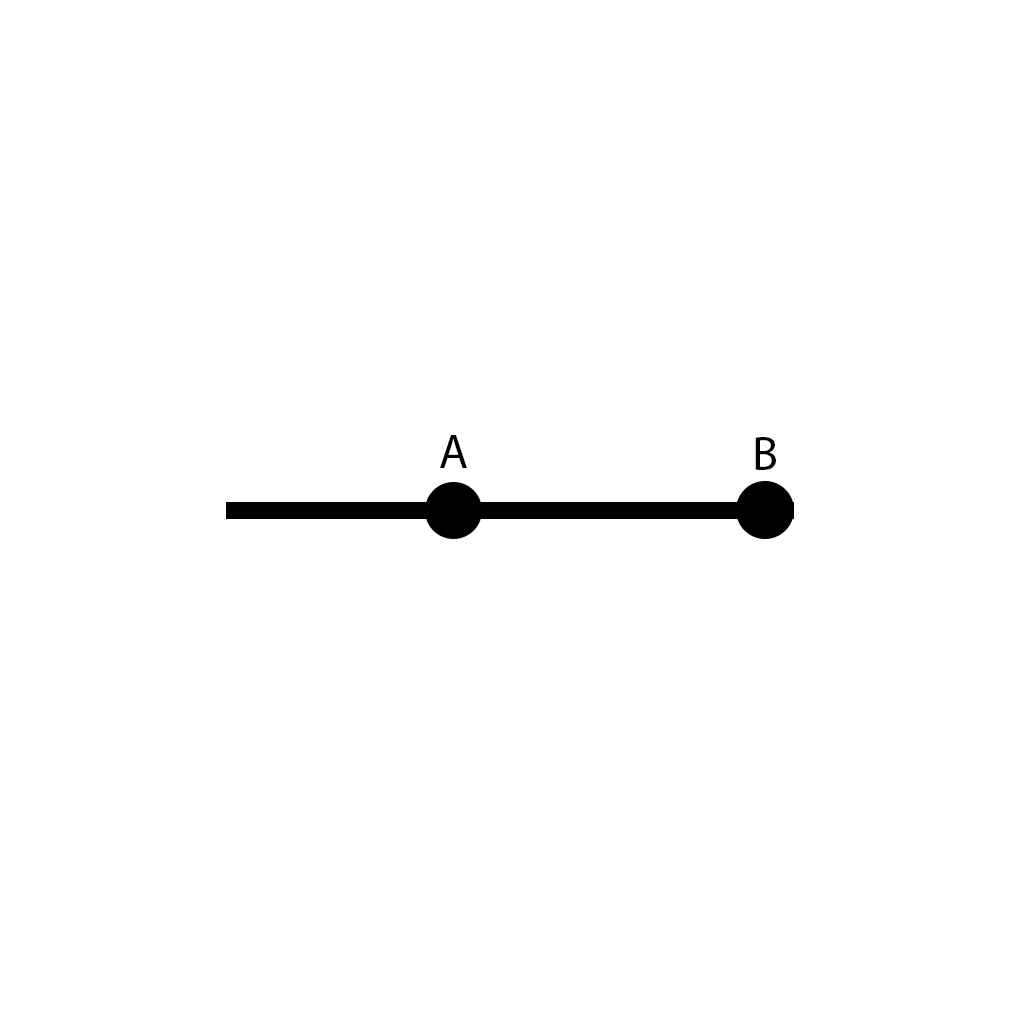
\includegraphics[width=\linewidth]{ALinear}
    \end{minipage}
    &
    \begin{minipage}{.22\textwidth}
      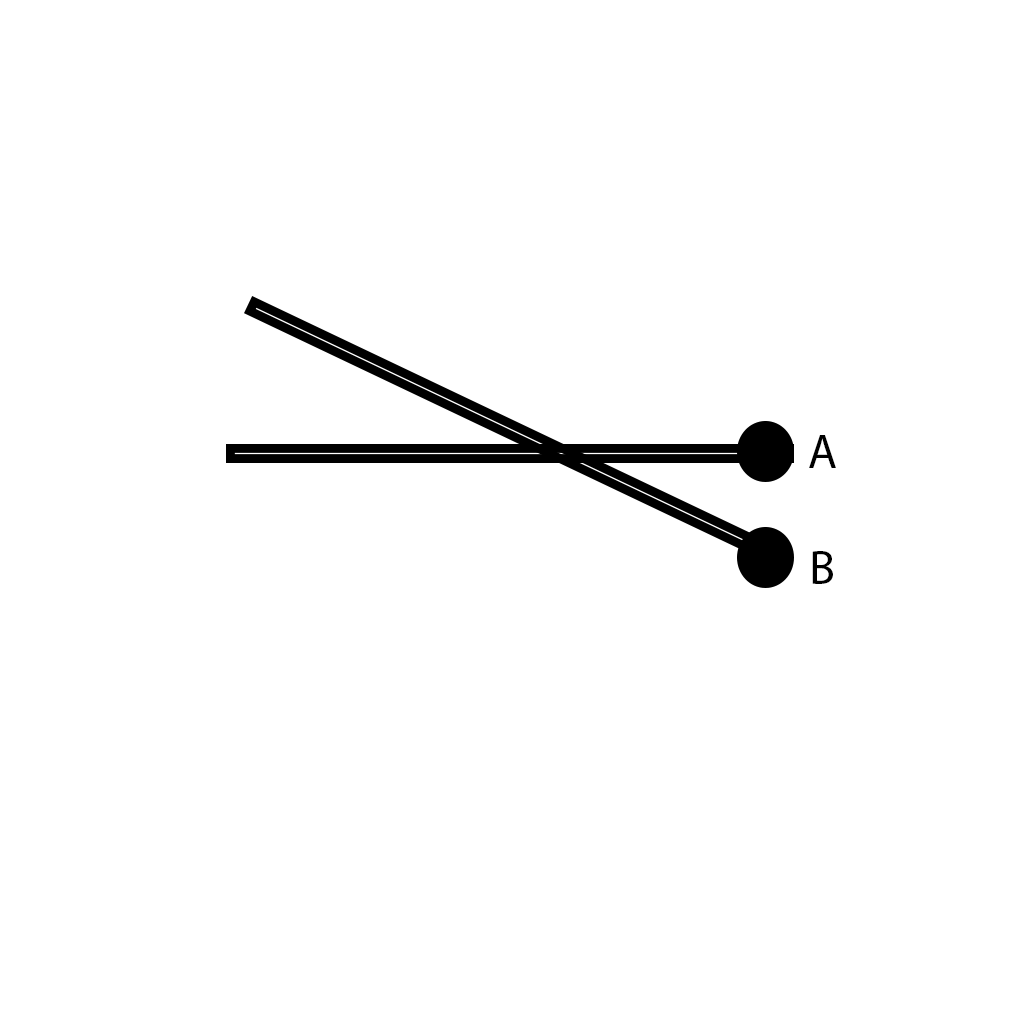
\includegraphics[width=\linewidth]{ILinear}
    \end{minipage}
    & 
    \begin{minipage}{.22\textwidth}
      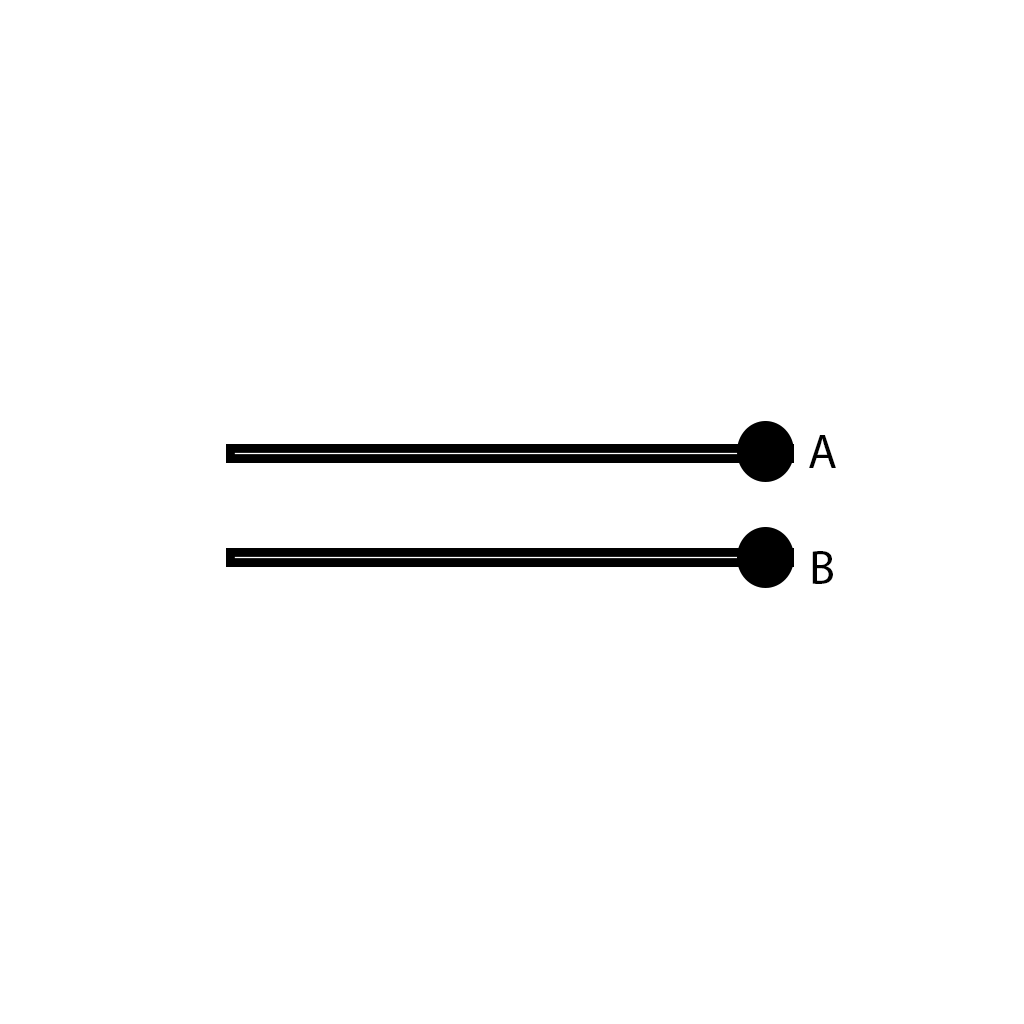
\includegraphics[width=\linewidth]{ELinear}
    \end{minipage}
    &
    \begin{minipage}{.22\textwidth}
      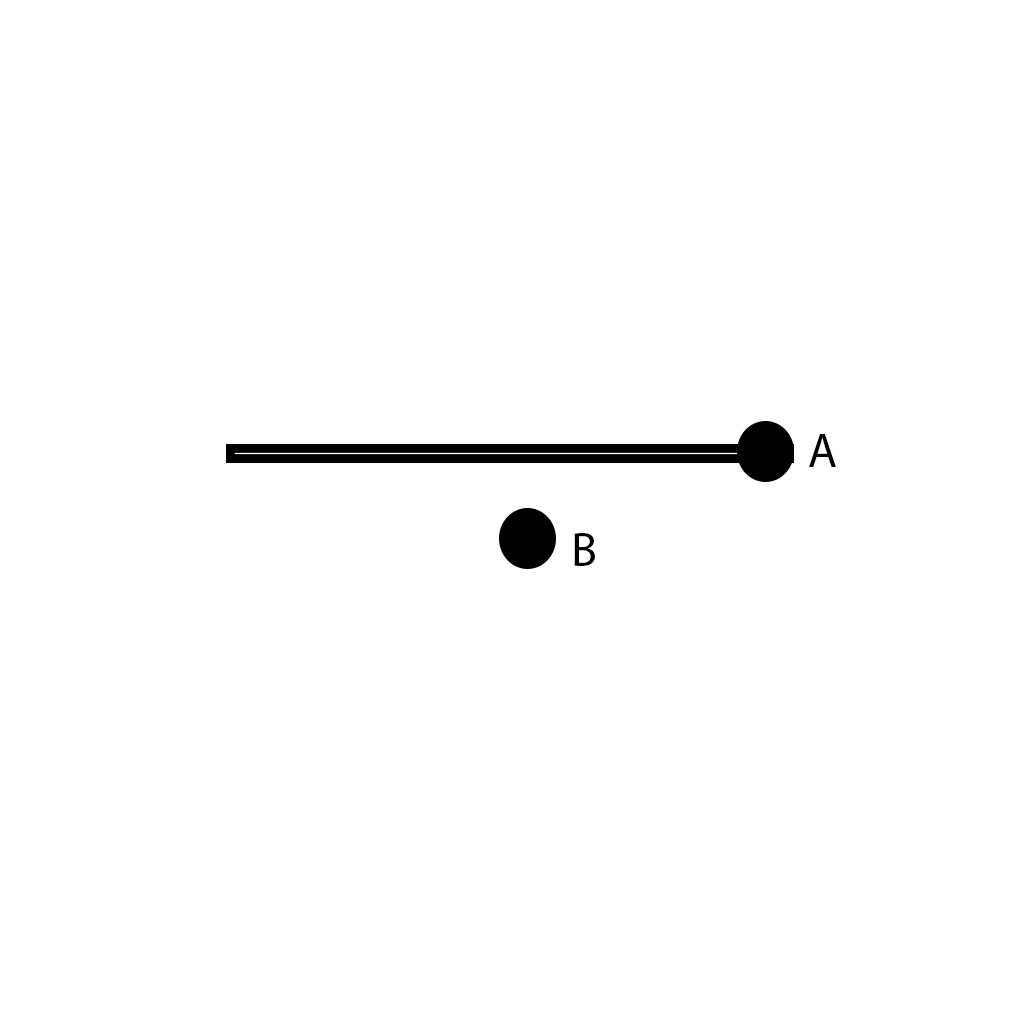
\includegraphics[width=\textwidth]{O1Linear}
    \end{minipage}
    \\
    &
     &
     &
    \begin{minipage}{.22\textwidth}
      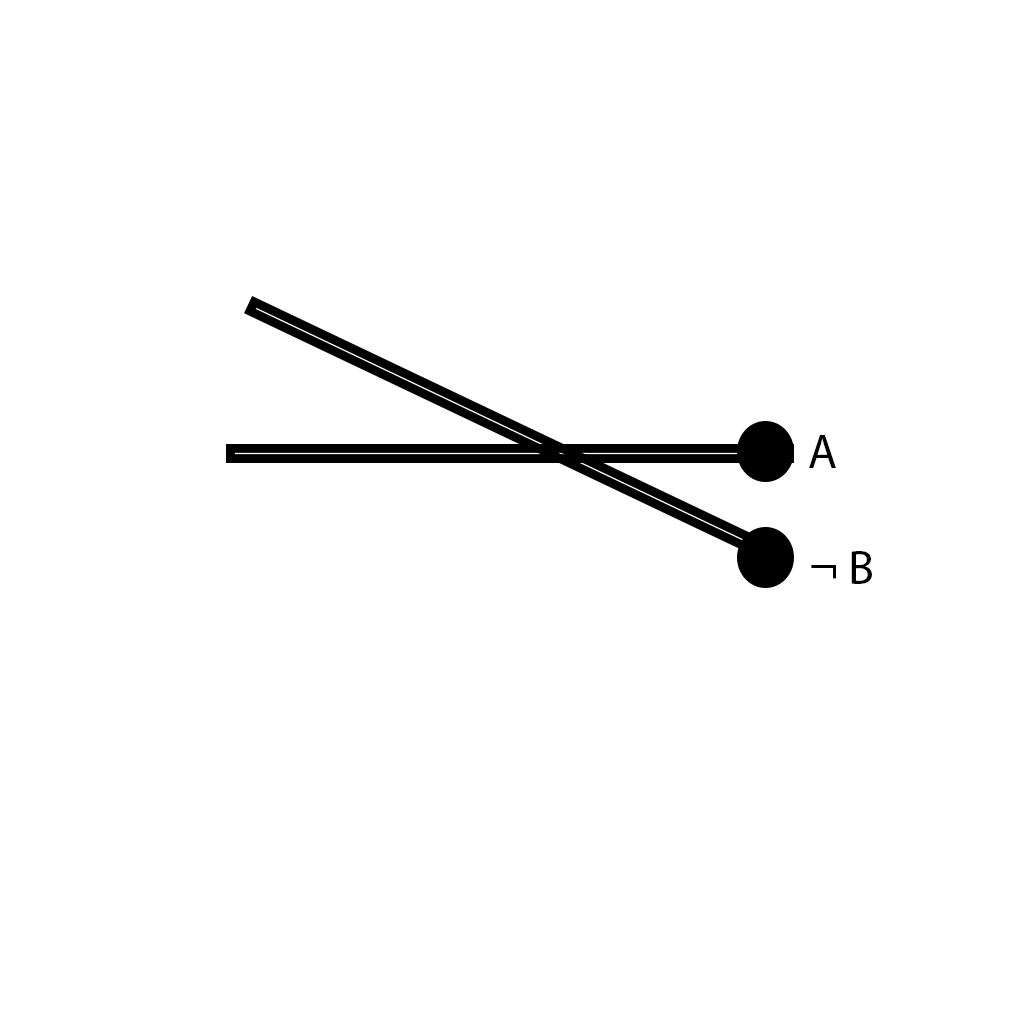
\includegraphics[width=\textwidth]{O2Linear}
    \end{minipage}
    \\
  \end{tabular}
  \caption{Premises represented by Linear Diagrams}\label{tbl:linearPremises}
\end{table}
\FloatBarrier

However, as shown by \cite{lemon1998insufficiency}, linear diagrams do not successfully manage to circumvent the same limitations that planar figures are susceptible to. \cite{lemon1998insufficiency} go as far to say that linear diagrams should only be used for trivial objects and relations and that they are unsuitable for more complex sets.

\subsection{Categorical Pattern Diagrams}
As introduced by \cite{cheng2012visualizing}, Categorical Pattern Diagrams offer a relatively new approach with regards to representing syllogisms. The aim behind them is to simplify the process of checking validity, better represent syllogisms with more than 2 premises and generally make the diagrams easier to infer from.

The issue with this form of representation is the notation used is not intuitive. Categorical Pattern Diagrams require the person to learn a whole new notation before they can begin to reason about the syllogism that it is representing.

\begin{table}[h!]
  \centering
  \begin{tabular}{  c  c  c  c }
    A & I & E & O\\
    \begin{minipage}{.22\textwidth}
      
\includegraphics[width=\linewidth, scale=0.5]{CPDA}
    \end{minipage}
    &
    \begin{minipage}{.22\textwidth}
      
\includegraphics[width=\linewidth, scale=0.5]{CPDI}
    \end{minipage}
    & 
    \begin{minipage}{.22\textwidth}
      
\includegraphics[width=\linewidth, scale=0.5]{CPDE}
    \end{minipage}
    &
    \begin{minipage}{.22\textwidth}
      
\includegraphics[width=\textwidth]{CPDO}
    \end{minipage}
    \\
  \end{tabular}
  \caption{Premises represented by Categorical Pattern Diagrams}\label{tbl:cpdPremises}
\end{table}
\FloatBarrier

\section{Additional Logic Systems}
So far the only formal logic system looked at has been syllogisms, but many more exist. There are number of systems that would be ideal to include in the syllogism game to allow the player to gain a broader understanding of formal logic.

\subsection{Polysyllogisms}
Polysyllogisms, unlike standard syllogisms, can contain more than 3 propositions. This poses a problem for many graphical representations, with traditional circular Venn diagrams being limited to 3 sets. As figure \ref{fig:4SetVenn} and \ref{fig:4SetVenn} show it is possible to represent more than 3 sets using different shapes but as the diagrams become exponentially more complex as sets are added it is quickly becomes impractical to use them.

As reasoned by \cite{cheng2014graphical}, linear and Euler diagrams also struggle with this problem. As both use spatial-overlap it means the diagrams can only represent a series of universal affirmative propositions as further propositions are nested in. As can be seen in table \ref{tbl:linearPremises} and \ref{tbl:eulerHomework} there are already multiple ways to represent syllogisms with 3 terms so it is easy to see how it would quickly become unmanageable as the number of propositions increases.

\begin{figure}[!h]
  \centering
  \begin{minipage}[b]{0.4\textwidth}
    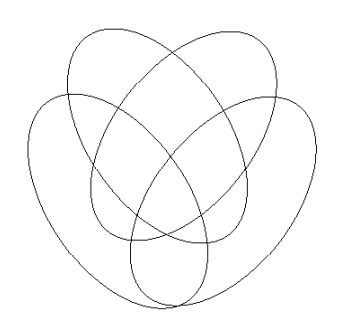
\includegraphics[width=\textwidth]{4SetVennDiagram}
    \caption{4 Set Venn Diagram}
    \label{fig:4SetVenn}
  \end{minipage}
  \hfill
  \begin{minipage}[b]{0.4\textwidth}
    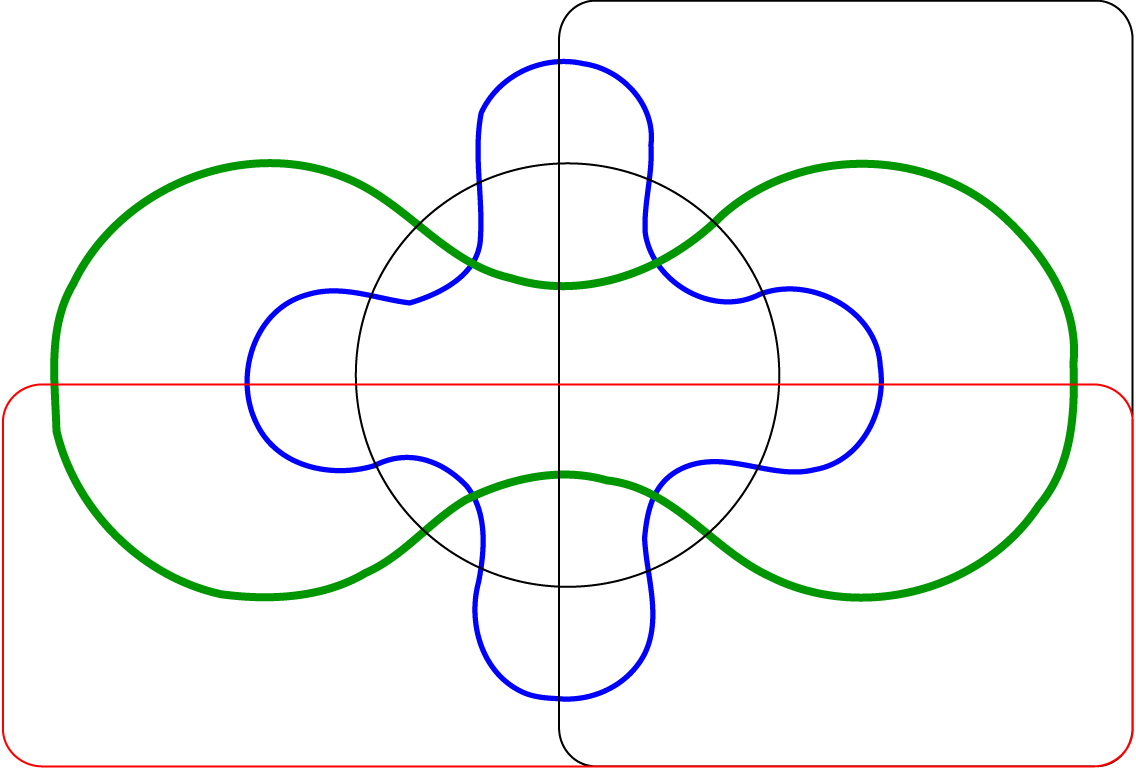
\includegraphics[width=\textwidth]{5SetVennDiagram}
    \caption{5 Set Venn Diagram}
    \label{fig:5SetVenn}
  \end{minipage}
\end{figure}
\FloatBarrier

\subsection{Modal Logic}
Modal logic is an extension of classical proposition logic that uses the modal operators \textit{it is possible that} and \textit{it is necessary that} to describe a way in which the rest of the proposition can be true  \citep{zalta1988basic}. Modal logic allows statements to be expressed that would otherwise not be possible in (propositional) classic logic as it is not possible to convey the prospect of events happening. The following are examples of modal propositions:

\bigbreak
\begin{tightcenter}
It is possible that it will snow tomorrow\\
It is necessary that it is either snowing here now or it is not snowing here now.\\
\end{tightcenter}
\bigbreak

The necessity operator is denoted by $\square$, whilst the possibility operator is represented by $\lozenge$.

\subsection{Temporal Logic}
Temporal logic is a formal system for specifying and reasoning about propositions with regards to time. It is often used in the formal verification of software systems to interpret concurrent events \citep{lamport1983good}. Temporal logic can be split into two subsections, linear and branching. Linear temporal logic represents time as a set of paths with each part being a sequence of moments. From any given moment there is only one possible future moment, a unique successor. Branching linear logic represents time as a tree with the root as the present and the branches being the future.


\begin{figure}[!h]
  \centering
  \begin{minipage}[b]{0.4\textwidth}
    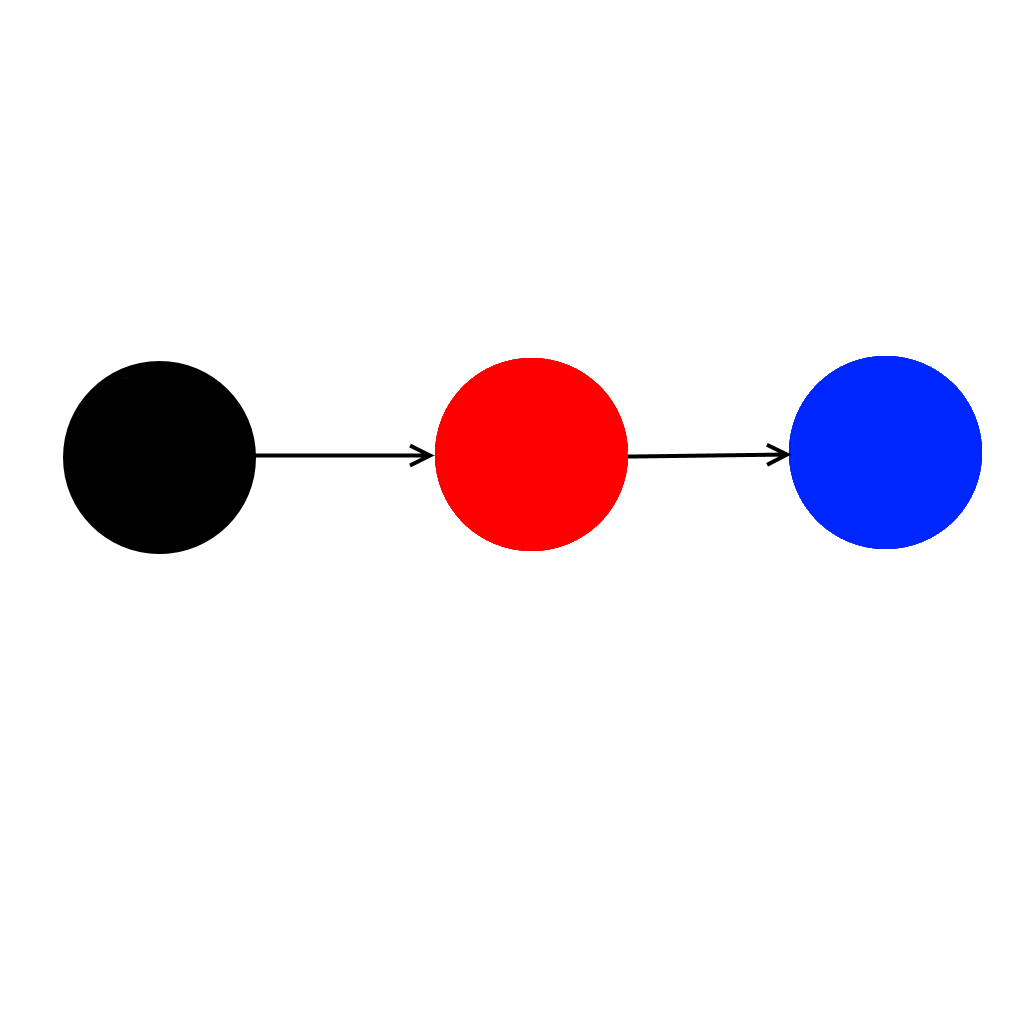
\includegraphics[width=\textwidth]{LinearTemporalLogic}
    \caption{Linear Temporal Logic}
  \end{minipage}
  \hfill
  \begin{minipage}[b]{0.4\textwidth}
    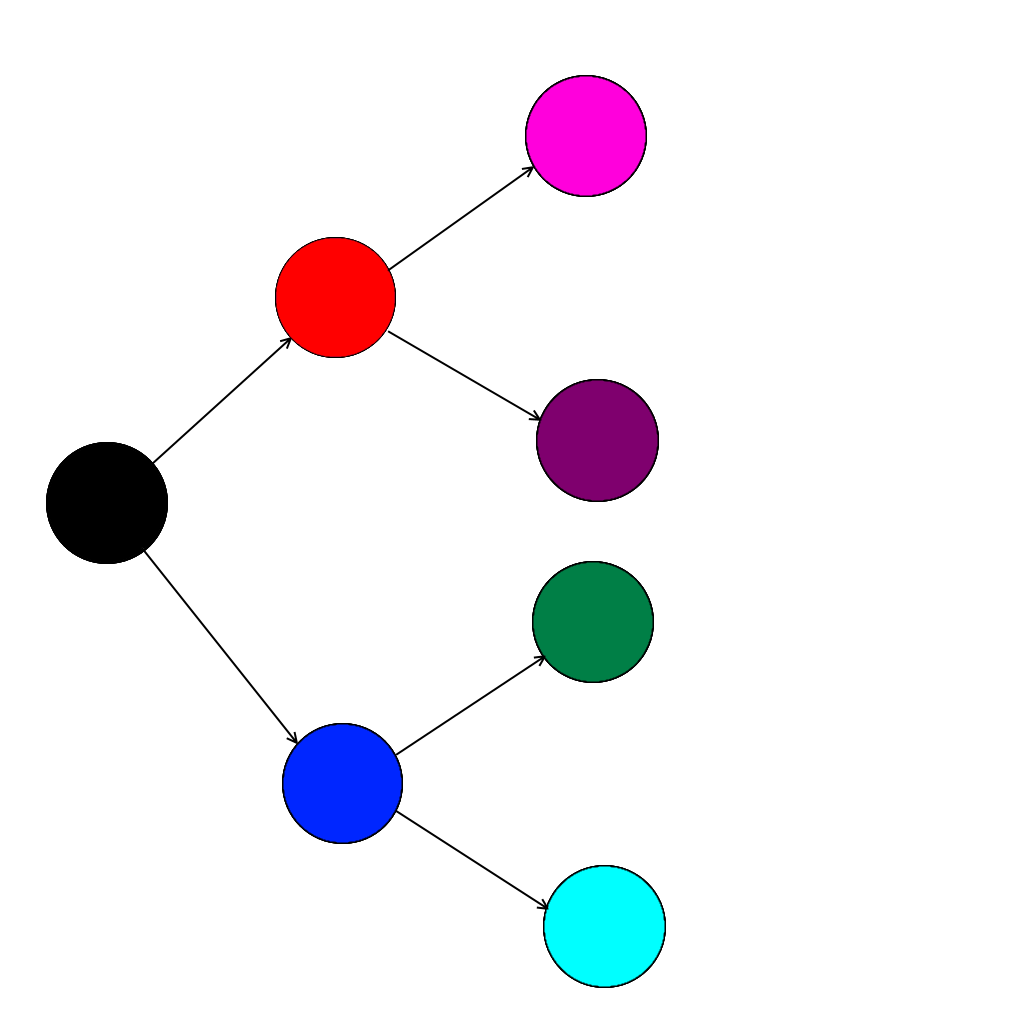
\includegraphics[width=\textwidth]{BranchingTemporalLogic}
    \caption{Branching Temporal Logic}
  \end{minipage}
\end{figure}
\FloatBarrier

\subsection{Set Theory}
Set theory is the mathematical theory of well-defined collections known as sets. These sets are made up of objects called elements. Given a set $S$ and an element $x$ it is said $x \in S$ if $x$ is an element of $S$ and conversely $x \notin S$ if $x$ is not an element of $S$ \citep{sep-set-theory}.

Diagrammatically they appear very similar to syllogisms as both utilise Venn diagrams so it would naturally follow on well to expand syllogisms to encompass set theory. This is especially true when it is considered how syllogisms can be represented using set theory notation as in table \ref{tbl:setTheoryNotationTable}.
 
\begin{table}[h!]
\begin{center}
  \begin{tabular}{ c | c | c }
    Syllogism & Set Notation & Sentential Representation \\ \hline
    AaB & $B \subseteq A$ & All B is A \\
    AiB & $B \cap A \neq \emptyset$ & Some B is A \\
    AeB & $B \cap A = \emptyset$ & No B is A \\
    AoB & $B \cap A \nsubseteq B$ & Some B is not A \\
  \end{tabular}
   \caption{Set Theory Notation for Syllogisms}
  \label{tbl:setTheoryNotationTable}
\end{center}
\end{table}


\chapter{Serious Games}
\section{Introduction}
Serious Games are a movement within the game industry comprised of software developers and researchers who are using games to educate. Whilst there is some debate around what exactly construes a serious game, \cite{michael2005serious} define one as any game where entertainment is not the primary purpose, but where instead the focus is on education. They aim to tackle a growing problem whereby educational techniques have not adapted to the needs of the current generation. As \cite{lim2008spirit} discusses, learning in the classroom has been driven by the national curriculum, with a massive focus on standard and grades. This goes against the belief that to attract the attention of students the focus should in fact be on creating an engaging learning environment. In contrast with previous generations, the younger generation of today have grown up in a world consumed in technology. \cite{oblinger2005educating} described them as the \textit{Net Generation}, the generation who always need to be connected, require immediate feedback and crave social interaction. The research of \cite{prensky2001games} explains how this vast amount of technology now experienced in everyday life has led to these newer generations having their minds rewired. These cognitive changes have caused a different set of educational preferences when compared to previous generations, with teaching methods not evolving in order to take this into account.

\section{Why They Are Good For Education}
\subsection{Accessibility}
One of the benefits of using games to teach is their accessibility in comparison to other methods. In the United Kingdom  access to the internet has doubled over the past 10 years, with 82\% of adults now using the internet on a daily basis \citep{onssurvey}. With such a huge number of people using the internet it means that games hosted on the web have an extremely large potential audience. This broad audience coupled with the widespread appeal of video games allows the crossing of demographic boundaries such as age, gender and educational status \citep{griffiths2002educational}.  Serious Games also have a lower barrier to entry than other educational techniques by allowing a much more "pick up and play" approach to learning with less reliance on prerequisite background knowledge. In the case of syllogisms this would be achieved by using graphical representations to replace the set theory notations. By teaching the concepts first, set theory notation could then be introduced at a more appropriate time in the learning process when the player had a greater understanding of the topic. 

\subsection{Motivation}
As discussed by \cite{malone1981toward} games can be intrinsically motivating, such that there are no external factors as to why a person is playing other than for their own enjoyment. This is in contrast to typical classroom learning that is usually more extrinsically motivated through grades, exam results and certificates. As  \cite{csikszentmihalyi1997talented} says, the school attendance would see a sharp drop if extrinsic rewards were removed. Of the two, intrinsic motivation is more resilient than extrinsic motivation and learning that takes place as a result of intrinsic motivation is of higher quality and longer lasting \citep{kawachi2003initiating}.

However, it is important to remember that not all games are by definition intrinsically motivating, but need to be structured correctly to achieve this. Malone included challenge, fantasy and curiosity as the three cornerstones of intrinsically motivating serious games.  
In order to create a challenging game, it should include uncertain goals that are not too easy for the players to complete. Ensuring a game is challenging is crucial as demonstrated by Malone's work surveying children's opinion on 25 different computer games. The results conclusively showed that the most popular games all shared one thing in common; they all contained a defined goal.  Similarly in a study carried out by \cite{abuhamdeh2012importance} on chess players, it was found that the more challenging the game the greater the player's enjoyment. This is important to bear in mind with syllogisms as it is demonstrates the need to add the correct amount of difficulty for the game to be successful.

A fantasy environment in a game is said to "evoke mental images of phyical or social situations not actually present". Malone divides these fantasies into intrinsic and extrinsic, with intrinsic being more interesting and instructional resulting in a  greater cognitive effect on learning. \cite{lepper1988motivational} explains how if learning takes place away from the functionality of the knowledge then this decontextualisation results in the learner becoming demotivated.  This can be tackled by using real world examples demonstrating how the concepts are applied. For syllogisms this can just be as simple as using actual examples that exist as opposed to using letters to represent sets. However, as this is not always feasible, Lepper proposed inserting the content of the topic into a fantasy context.
Curiosity, like challenge, is stimulated from an optimal level of complexity. Curiosity is also broken down into two categories; sensory and cognitive.  Sensory curiosity, as the name suggests, uses lights, sounds and graphics to gain the attention of the participant. Cognitive curiosity is achieved by making the participant doubt their existing knowledge, as people desire to have "good form" in their cognitive structure.   By using this taxonomy when developing a serious game, it is clear that this could be used to engage people who otherwise might not have been interested in learning. 

\subsection{Feedback}
Feedback is information regarding a person's understanding of a concept provided with the intention of improving the person's ability. Feedback is a crucial part of the education process and significantly influences the effectiveness of learning.

As stated by \cite{hattie2007power}, "feedback is
one of the most powerful influences on learning and achievement". A further study explored the most effective medium to provide feedback. Computer-assisted, audio and video feedback were found to be most effective forms with the more traditional approach of praise, punishment and providing extrinsic rewards being the worst \citep{hattie2007power}. 

One of the main advantages of using games for education is the speed at which feedback can be delivered to the learner which is especially important to the \textit{Net Generation}. The term \textit{fast feedback} was coined by \cite{lumsden1988characteristics} to demonstrate how this timely feedback removed any uncertainty about progress and allowed any corrective action to be taken during the learning process. However, fast feedback is not a silver bullet and as such the speed at which feedback is delivered should depend on the difficulty of the task. The more complex the task, the greater the benefit of delaying the feedback to allow the information to be processed \cite{clariana2000applying}. 

Feedback during the learning process is known as formative assessments, with summative assessments usually being carried out at the end. As explained by \cite{irons2007enhancing}, formative assessments can be beneficial as they enhance the learning process by creating a positive environment which results in greater motivation for learner. 

Serious Games lend themselves extremely well to delivering formative feedback to players through in-game features such as progress bars, score count and countdown timers. Feedback can also be provided to the player as they make mistakes allowing the player to engage with the game and keep on track to completing their goals. This can also help the player from becoming frustrated and unable to progress.

\section{Existing Serious Games}
Serious Games can be split into two main categories, mini-games and complex games. Mini Games tend to be far shorter, often only taking less than an hour to complete. The focus is aimed at a very specific topic within a subject and is usually browser based. Progression tends to be added through multiple levels, all with similar design but with increasing difficulty. This is the far more common type of Serious Game as they are far cheaper to develop.

In contrast, complex games can take potentially hundreds of hours to complete and cover a very broad topic. The game may contain multiple skills, paths to follow and complex goals.  

Serious games do not just apply to education, but are used by a wide variety of different industries. The United States military created America's Army to aid in their recruitment and Microsoft's Flight Simulator is used by pilots in training \citep{111701519980901}.


\subsection{MyMaths}
MyMaths is a web based service that is used by schools in over 70 countries, with over 4.5 million users. It is marketed as an online learning platform that provides lessons and homework to school children. It allows them to complete all of this work online and is then automatically marked.
As Figure 2.1 shows, MyMaths makes use of fast feedback to provide the player with the results as soon as they have completed the task. However, MyMaths does not provide an immersive or particularly enjoyable experience for players. \cite{lee2013learning} found that while students said they enjoyed using computers to learn, they did not want to use MyMaths. This could be due to that fact that MyMaths is very one dimensional, merely presenting questions in a quiz like format. This does not engage with the player, incite any emotive feelings or provide any fantasy environment. It would more enjoyable if the technologies available were used to make it more interactive.
\begin{figure}[!tbp]
  \centering
  \begin{minipage}[b]{1\textwidth}
    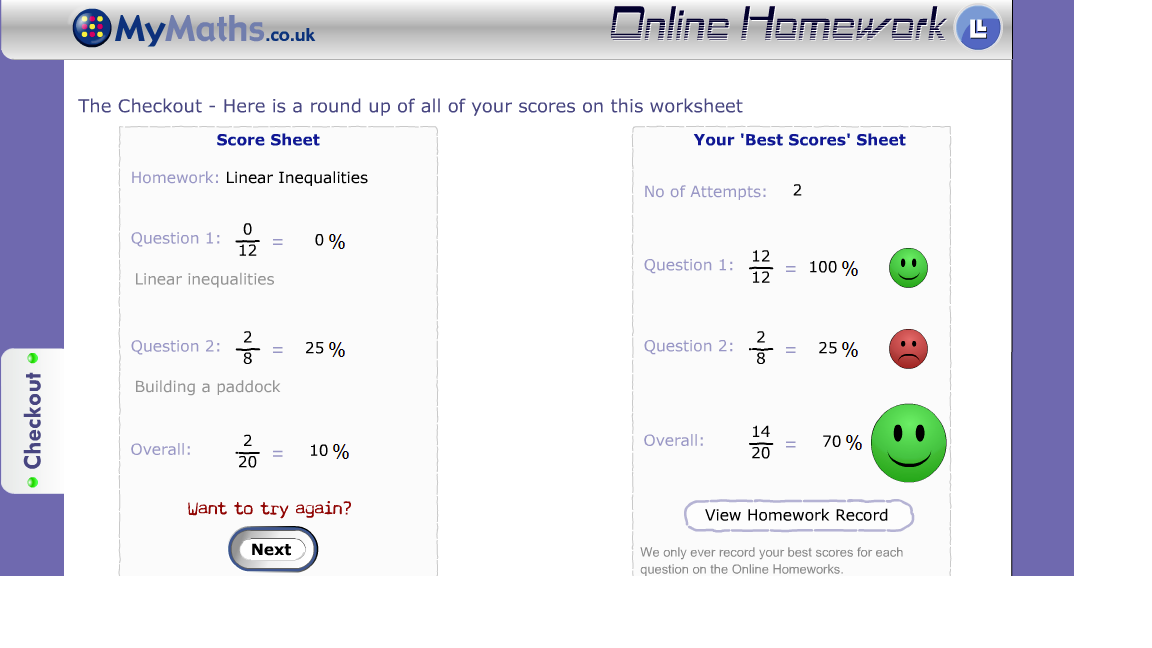
\includegraphics[width=\textwidth]{mymaths}
    \caption{A homework exercise in MyMaths}
  \end{minipage}
\end{figure}
\FloatBarrier

\bibliographystyle{plainnat}
\bibliography{bibliography} 

\end{document}